\documentclass[../review_3.tex]{subfiles}
\begin{document}

\chapter{Auswertung der erfassten Arbeitszeiten}\thispagestyle{fancy}
Mithilfe des  Zeiterfassungssystems Kimai können Arbeitszeiten der Teammitglieder erfasst werden. Dabei werden nicht nur der Beginn und das Ende der Bearbeitung einer Projektaufgabe von der Software aufgenommen, sondern es wird dieser auch eine passende Aktivitätskategorie und fakultativ ein kurzer Text hinzugefügt. Die verschiedenen Kategorien sind in diesem Projekt:
\begin{itemize}
    \setlength{\parskip}{-0.2pt}
    \item Administration (z.B. Aktualisieren des Gantt-Diagramms)
    \item Entwurf (z.B. Erstellen des Klassendiagramms oder der Aktivitätsdiagramme)
    \item Dokumentation (z.B. Arbeiten am Review-Dokument)
    \item Implementierung (z.B. Programmieren einer konkreten Klasse)
    \item Installation (z.B. Herunterladen von DPDK)
    \item Meetings (z.B. Montagsmeeting mit dem Betreuer um 18:30 Uhr)
    \item Präsentationsvorbereitung (z.B. Erstellen der Präsentationsfolien)
    \item Recherche (z.B. Vergleichen verschiedener Maps durch Reports im Internet)
    \item Test (z.B. Ausführen von Unit Tests und anderen Tests)
\end{itemize}
Mithilfe dieses Tools kann somit jedes Teammitglied regelmäßig einen Überblick erhalten, was es wann wie lange für das Software-Projekt gearbeitet hat. \\
Am Ende jeder der drei Phasen (Planung- und Entwurf, Implementierung, Validierung) werden die vom Kimai erfassten Daten ausgewertet. Dies ermöglicht die Identifikation von Problemen und das Vorbeugen eventuell später aufkommender Komplikationen. Falls sich somit in der Auswertung Probleme zeigen, werden Verbesserungsvorschläge und Gegenmaßnahmen entwickelt. \\
In diesem Kapitel werden die bisher erfassten Zeiten analysiert und in Diagrammen dargestellt. Diese Diagramme wurden automatisch aus den Daten einer Excel-Datei generiert. Diese Daten stimmen mit denen aus dem Kimai überein.

Den drei Phasen wurden folgende Kalenderwochen zugeordnet:
\begin{itemize}
    \item Planungs- und Enturfsphase: KW 17 - KW 21
    \item Implementierungsphase: KW 22 - KW 24
    \item Validierungsphase: KW 25 - KW 28
\end{itemize}
Anmerkung: Die Kalenderwoche 29 wird nicht ausgewertet, da diese durch die Abgabe des Reviewdokumentes am Mittwoch nicht vollständig ausgewertet werden kann.

Die Phasen werden in den folgenden Kapiteln einzeln ausgewertet und deren Ergebnisse am Ende verglichen.
\section{Planungs- und Entwurfsphase}

Die folgenden Auswertungen wurden direkt nach Ende der Planungs- und Entwurfsphase vorgenommen.

\begin{figure} [h]
    \centering
    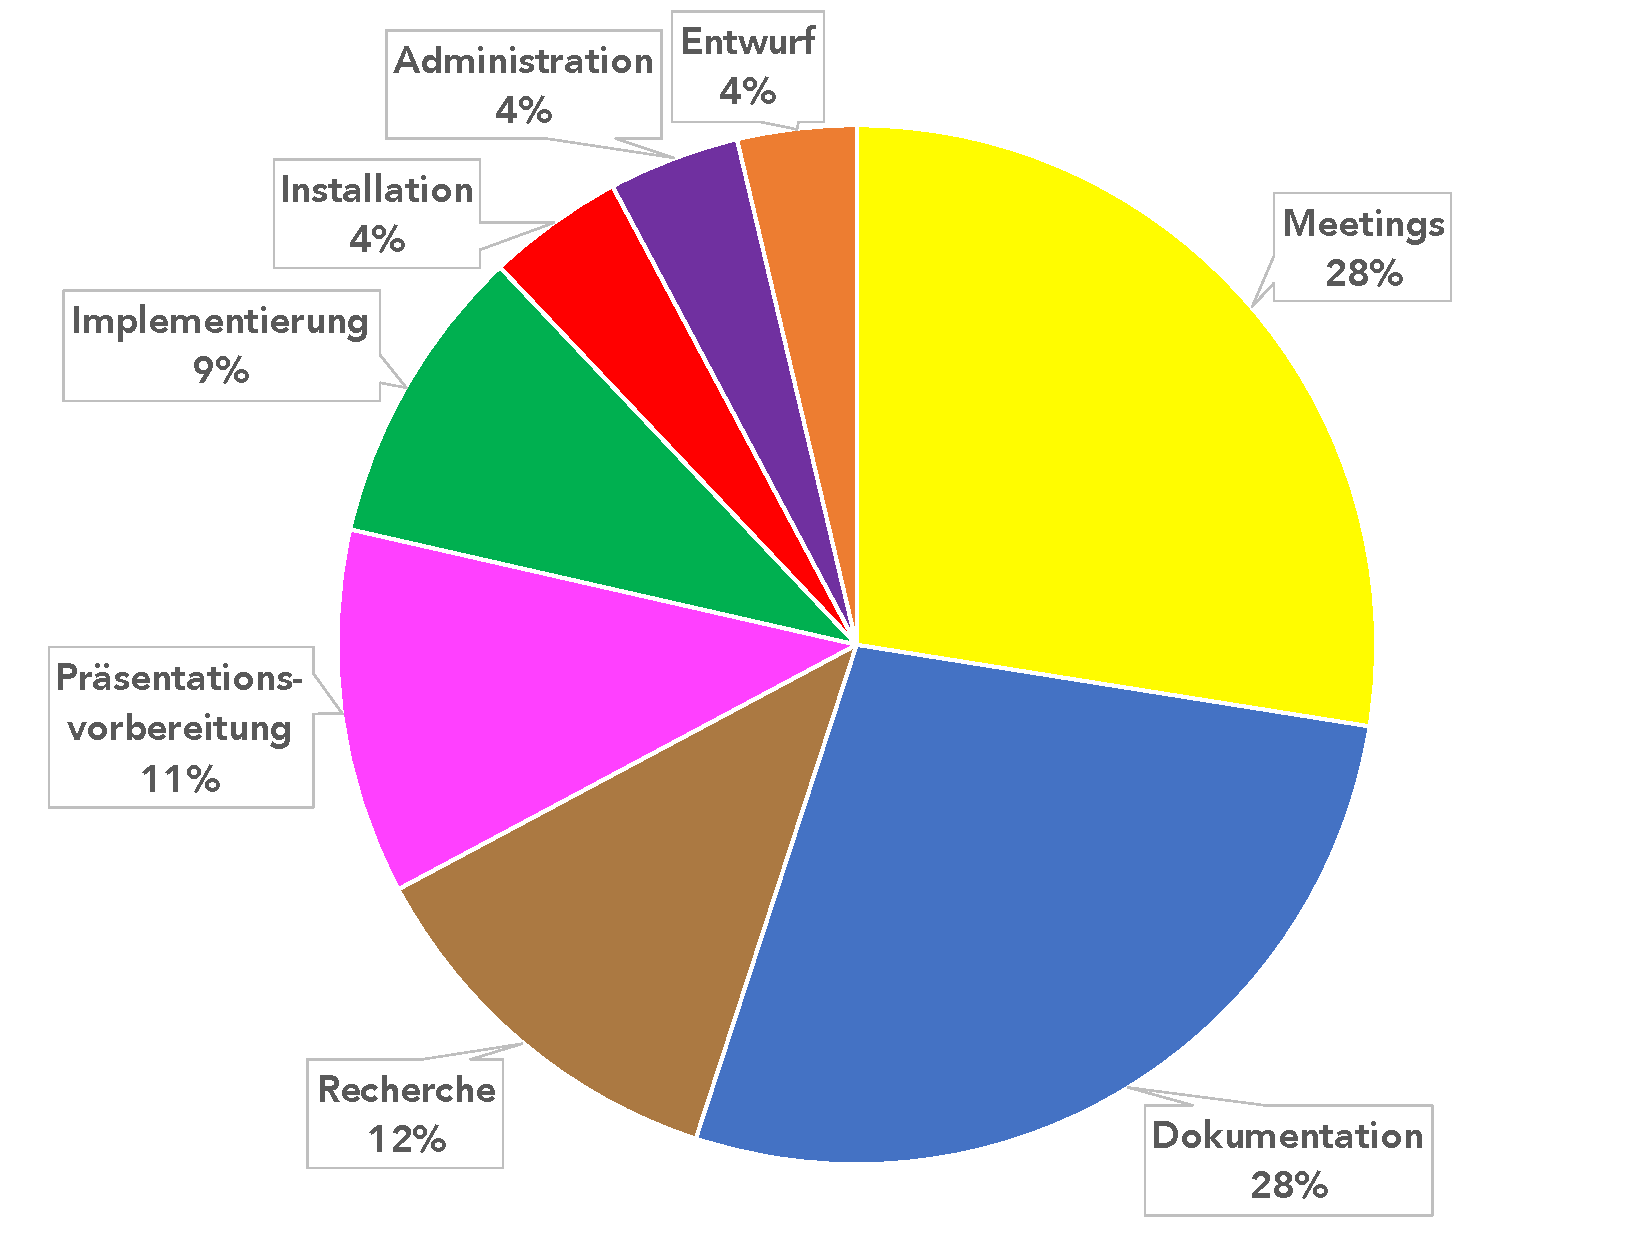
\includegraphics[width = 0.8 \linewidth]{img/Kimai1.pdf}
    \caption{Planungs- und Entwurfsphase (KW 17-21): Anteile der Aufgabenkategorien an der insgesamt aufgebrachten Zeit}
    \label{kategorien}
\end{figure}

Das Diagramm \ref{kategorien} zeigt, dass die Zeit in der Planungs- und Entwurfsphase vorwiegend für \textbf{Meetings} aufgewendet wurde. Der Grund dafür könnten die häufigen langen Diskussionen in den Meetings mit allen Teammitgliedern sein. Zudem wurde oft die gemeinsame Arbeit an Aufgaben ebenfalls als Meeting gebucht, auch wenn eine andere Kategorie besser gepasst hätte. Beispielsweise wurde das Klassendiagramm in den wöchentlichen Meetings gemeinsam entworfen. Diese Entwurfsaktivität wurde hier aber unter Meetings und nicht unter Entwurf verbucht. Lösungsideen sind, Meetings themenspezifischer zu buchen und diese nach Möglichkeit in kleineren Gruppen abzuhalten, falls die Themen nicht alle Mitglieder betreffen. Jedoch ist zu beachten, dass hierbei die Konsistenz gewahrt wird. Das bedeutet, dass die \glqq großen\grqq{} Meetings mit dem gesamten Team weiterhin unter Meetings verbucht werden müssen. Dies wurde sowohl bei einem Meeting als auch durch einen Eintrag im Wiki allen Teilnehmern des Projekts kommuniziert. Weiterhin könnten weniger bzw. kürzere Meetings gehalten werden und detaillierte Fragen direkt mit den zuständigen Personen geklärt werden. Dies dann entweder in einem eigenen Meeting oder über die Plattform Zulip.

Außerdem wurde mit 26\% viel Zeit für die Kategorie \textbf{Dokumentation} in Anspruch genommen. Ein möglicher Grund dafür ist, dass auch die Arbeit am Entwurf (z.B. am Klassen- oder Paketdiagramm) und die dazugehörige Entwurfsdokumentation nur unter der Kategorie Dokumentation, nicht aber unter der Kategorie Entwurf gebucht wurde. Daraus ergibt sich, dass das Team in Zukunft detaillierter buchen soll und die Kategorien womöglich angepasst werden muss.
Die für die \textbf{Recherche} aufgebrachte Zeit ist tendenziell verhältnismäßig und bedarf keiner Änderung.

Es fällt auf, dass für die \textbf{Vorbereitung} von Präsentationen  mit 11\% in dieser Projektphase vergleichsweise viel Zeit aufgewendet wurde. Dies resultiert daraus, dass jedes Teammitglied in der ersten Woche eine Präsentation zu verschiedenen Themen wie DoS-Angriffen oder DPDK gehalten hat und eine Vorlage für Präsentationen erarbeitet werden musste. Im weiteren Verlauf des Projektes sollte dieser Anteil sinken, da dann nur noch eine Präsentation pro Phase gehalten werden muss. Zudem müssen womöglich weniger Grafiken für das Review erstellt werden und das Präsentationsdesign kann wiederverwendet werden.

Für die \textbf{Installation} sind 6\% der Zeit aufgebracht worden. Auch dieser Wert sollte im Verlauf sinken, weil ein Großteil der Installationen bereits erfolgt sind.

In der Planungs- und Entwurfsphase war der Zeitaufwand für die \textbf{Implementierung} sehr gering, was zu Beginn des Projektes allerdings kein Problem darstellt, da hier lediglich ein erster Prototyp mit stark reduziertem Funktionsumfang entwickelt wurde. Zudem kann es daraus resultieren, dass in dieser Phase mit der Implementierung lediglich zwei der acht Teammitglieder beauftragt waren. Es wird erwartet, dass mit Beginn der Implementierungsphase der für die Implementierung erfasste Aufwand sprunghaft ansteigt.

Der geringe Anteil des \textbf{Administrationsaufwandes} ist positiv zu bewerten, weil er auf eine effiziente Planung und Verwaltung hinweist.

Die 3\% der erfassten Zeit, die der \textbf{Entwurf} in Anspruch genommen hat, sind zu wenig. Das ist wahrscheinlich darauf zurückzuführen, dass andere Kategorien für Arbeiten am Entwurf beim Buchen verwendet wurden, beispielsweise Dokumentation oder Meetings (Erklärung siehe oben).

\begin{figure} [h]
    \centering
    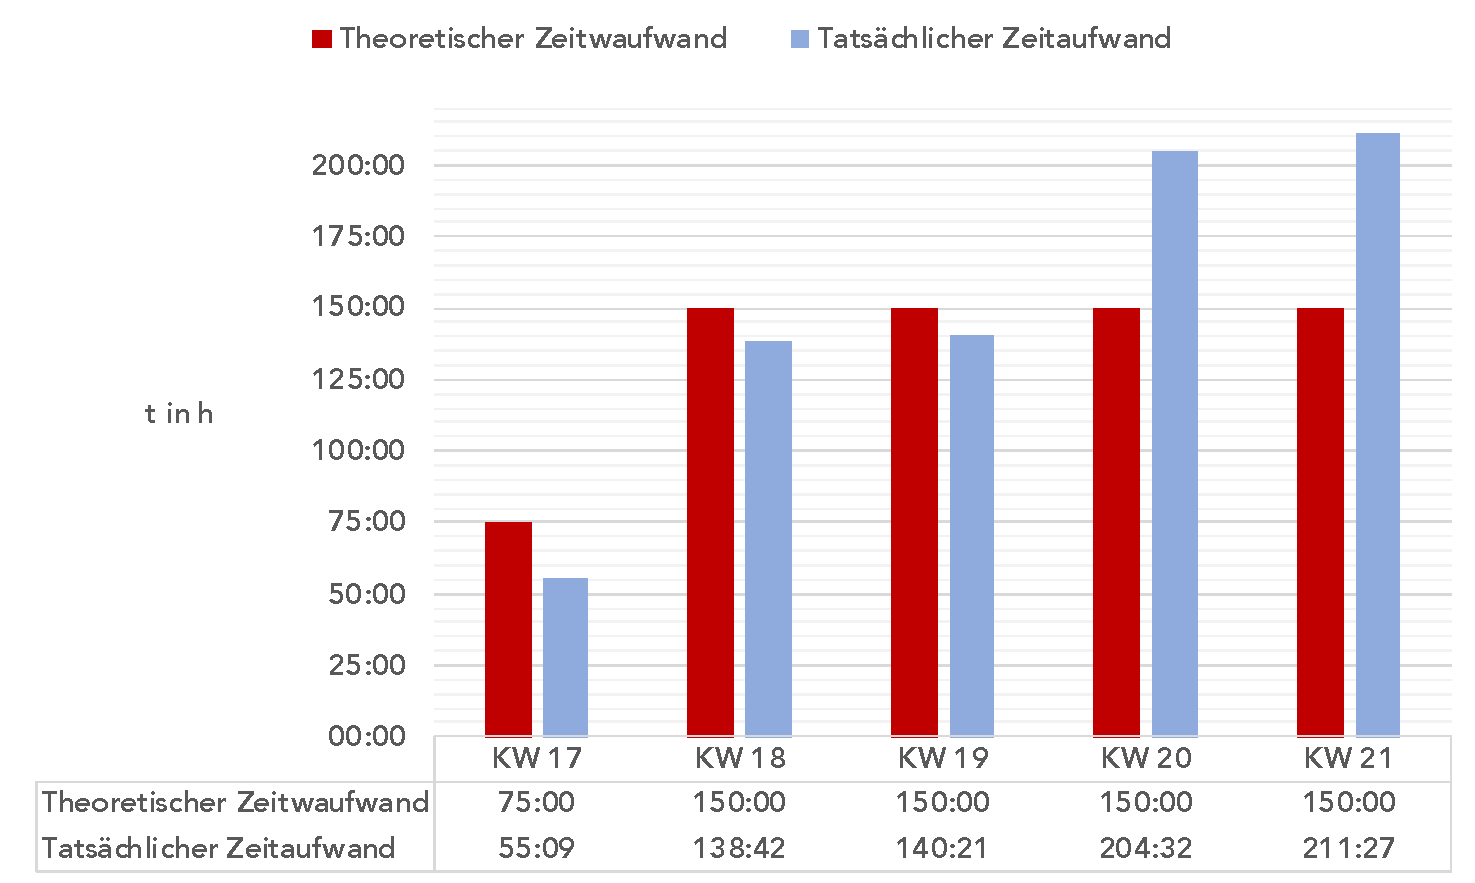
\includegraphics[width = \linewidth]{img/Kimai2.pdf}
    \caption{Planungs- und Entwurfsphase (KW 17-21): Vergleich des theoretischen Aufwands mit dem tatsächlichen Aufwand}
    \label{sollist}
\end{figure}

Im Balkendiagramm in \ref{sollist} wird dem theoretischen Zeitaufwand pro Woche der tatsächliche Aufwand gegenübergestellt. Die hier angegebenen tatsächlichen Zeiten ergeben sich aus der Addition der wöchentlichen Zeiten aller Teammitglieder.
Während Informatiker und Ingenieurinformatiker für das Softwareprojekt acht Leistungspunkte angerechnet bekommen, beträgt diese Punktzahl bei Wirtschaftsinformatiker lediglich sechs. Deshalb wird als Richtwert für die aufzubringende Zeit pro Woche zwischen den Studiengängen unterschieden: Bei Informatikern und Ingenieurinformatikern beträgt dieser Wert 20 Wochenstunden, bei Wirtschaftsinformatikern dagegen nur 15 Wochenstunden.
Da das Team aus vier Informatikern, zwei Ingenieurinformatikern und zwei Wirtschaftsinformatikern besteht, beträgt der Soll-Wert pro Woche 150 Stunden.
\begin{equation*}
    2\cdot 20h + 4\cdot 20h + 2\cdot 15h = 150h
\end{equation*}
In Woche 17 liegt Soll-Wert nicht bei 150 Stunden, sondern bei 75 Stunden, da das Projekt erst am Donnerstag begonnen hat und somit diese Woche kürzer als die anderen war.

In dieser Kalenderwoche liegt der Ist-Wert fast 20 Stunden unter diesen 75 Stunden, nämlich bei 55 Stunden und 9 Minuten. Dieses Defizit ist darin zu begründen, dass in dieser ersten Woche das Zeiterfassungssystem den Teammitgliedern noch nicht zur Verfügung stand. Deshalb mussten die Zeiten in der kommenden Woche nachgetragen werden, was jedoch nicht vom gesamten Team gemacht wurde.

In der Kalenderwoche 18 und der Kalenderwoche 19 liegt der tatsächliche Wert nur noch knapp unter den angestrebten 150 Stunden.

In den beiden letzten Wochen der ersten Phase werden diese 150 Stunden sogar stark übertroffen.
Somit lässt sich generell ein positiver Trend ablesen. Es wird jedoch erwartet, dass der in der kommenden Projektphase aufgebrachte Aufwand nicht weiter stark ansteigen wird, da es neben dem Softwareprojekt noch zahlreiche andere Aufgaben für das Studium zu erledigen gibt. Somit ist es für die meisten Studierenden kaum möglich, mehr als 20 bis 30 Stunden für dieses Projekt in Anspruch zu nehmen.

\begin{figure} [h]
    \centering
    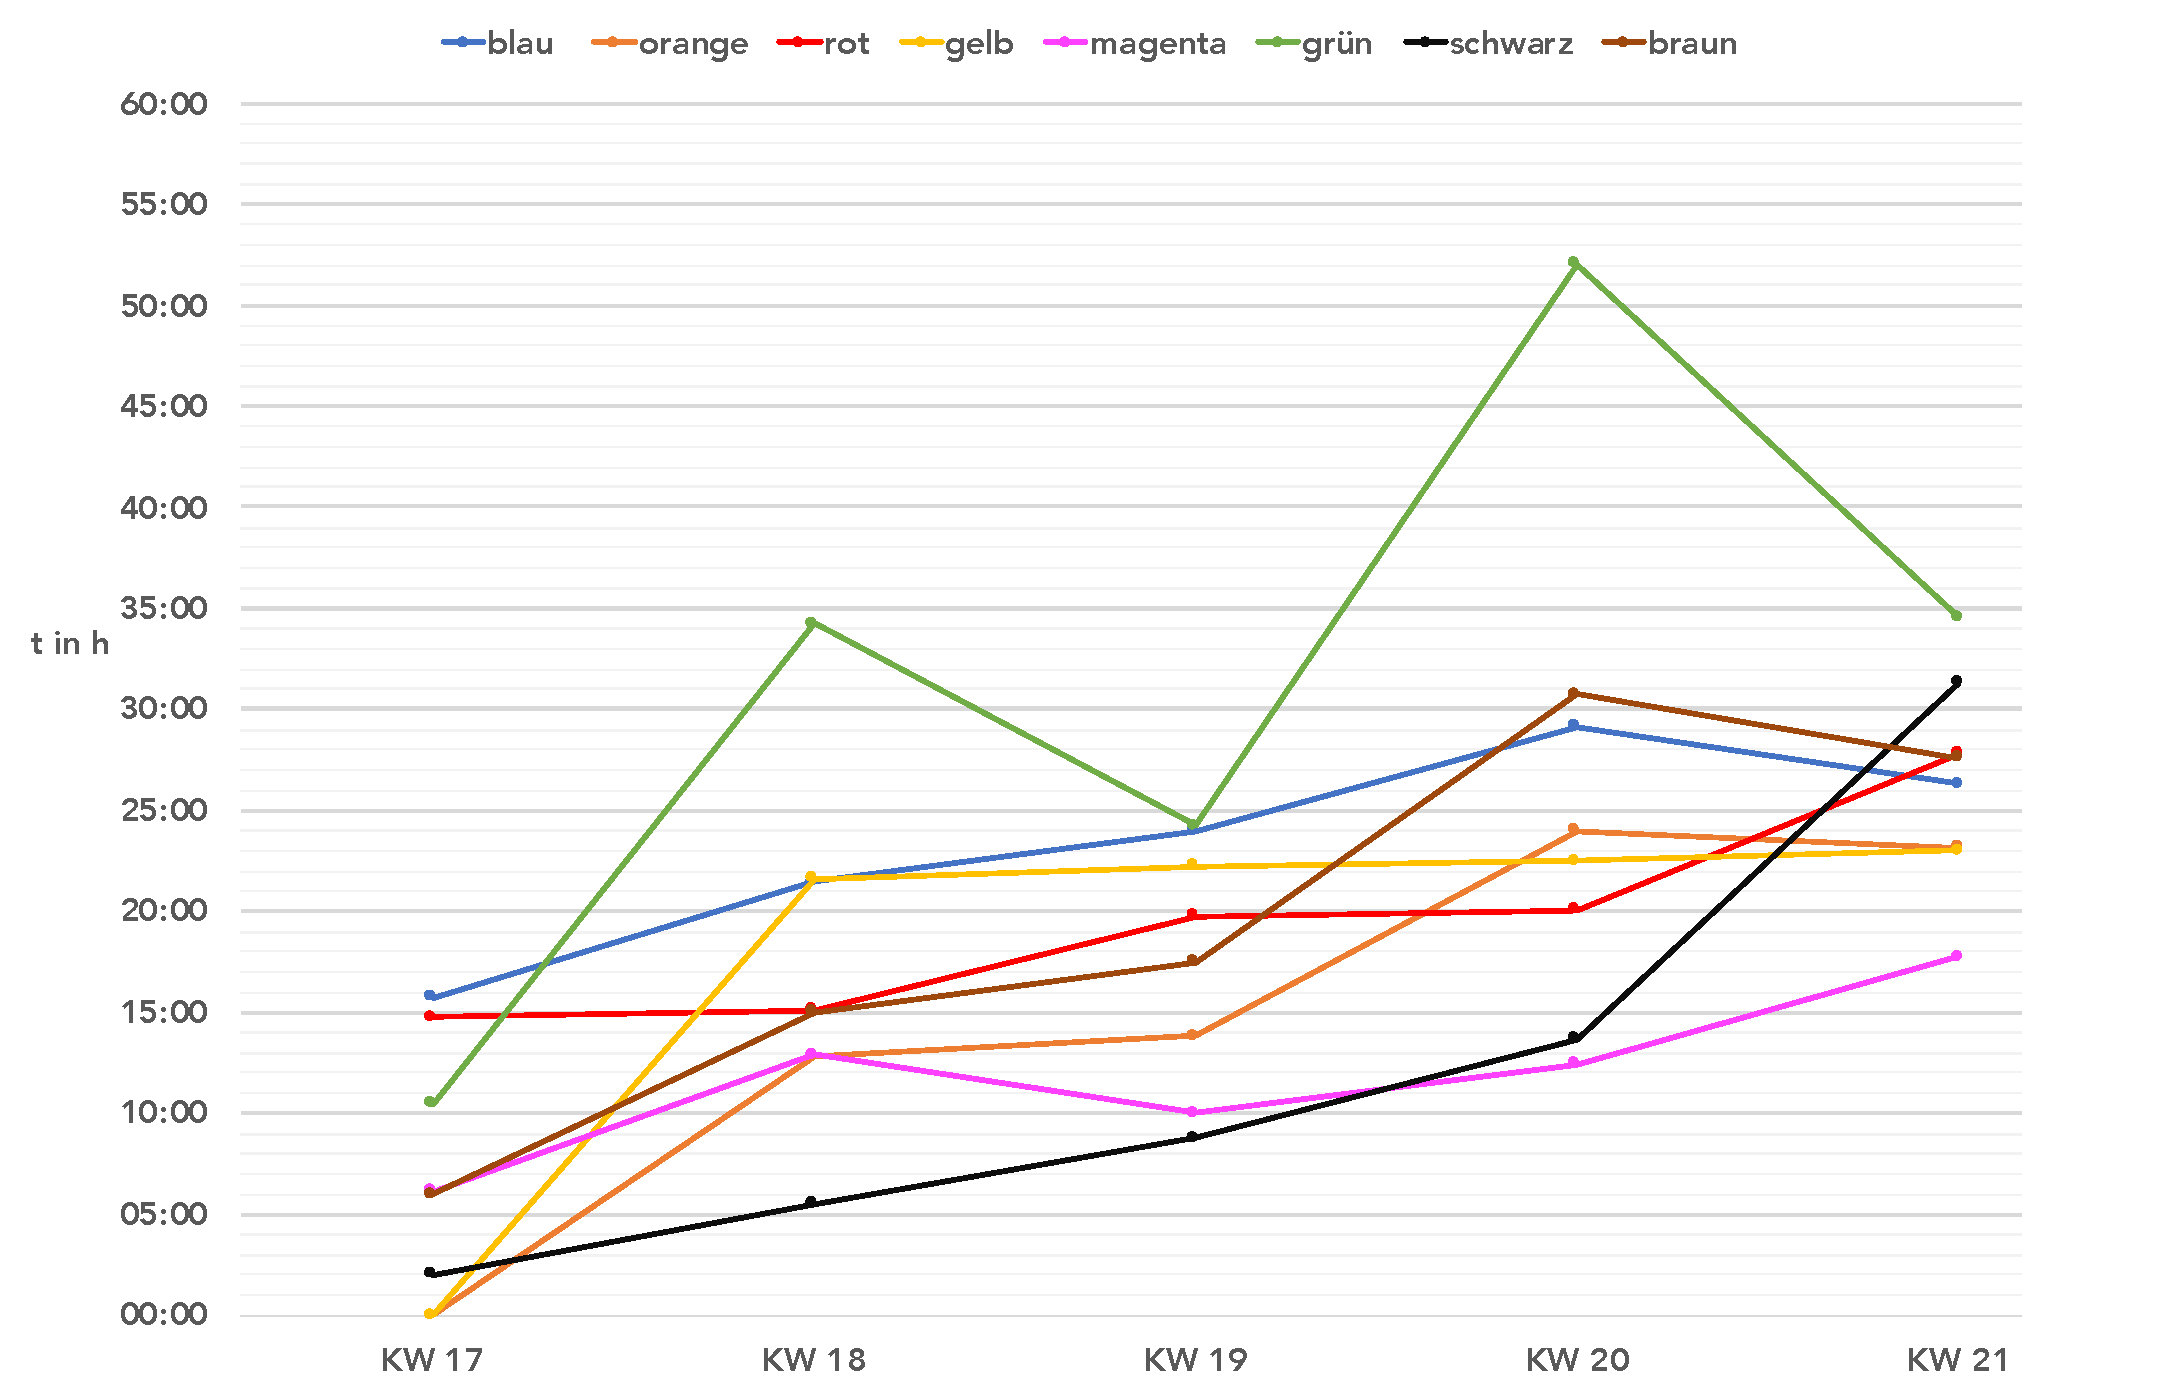
\includegraphics[width = \linewidth]{img/Kimai3.pdf}
    \caption{Planungs- und Entwurfsphase (KW 17-21): Zeitaufwand der einzelnen Teammitglieder}
    \label{teammitglieder}
\end{figure}

\begin{figure} [h]
    \centering
    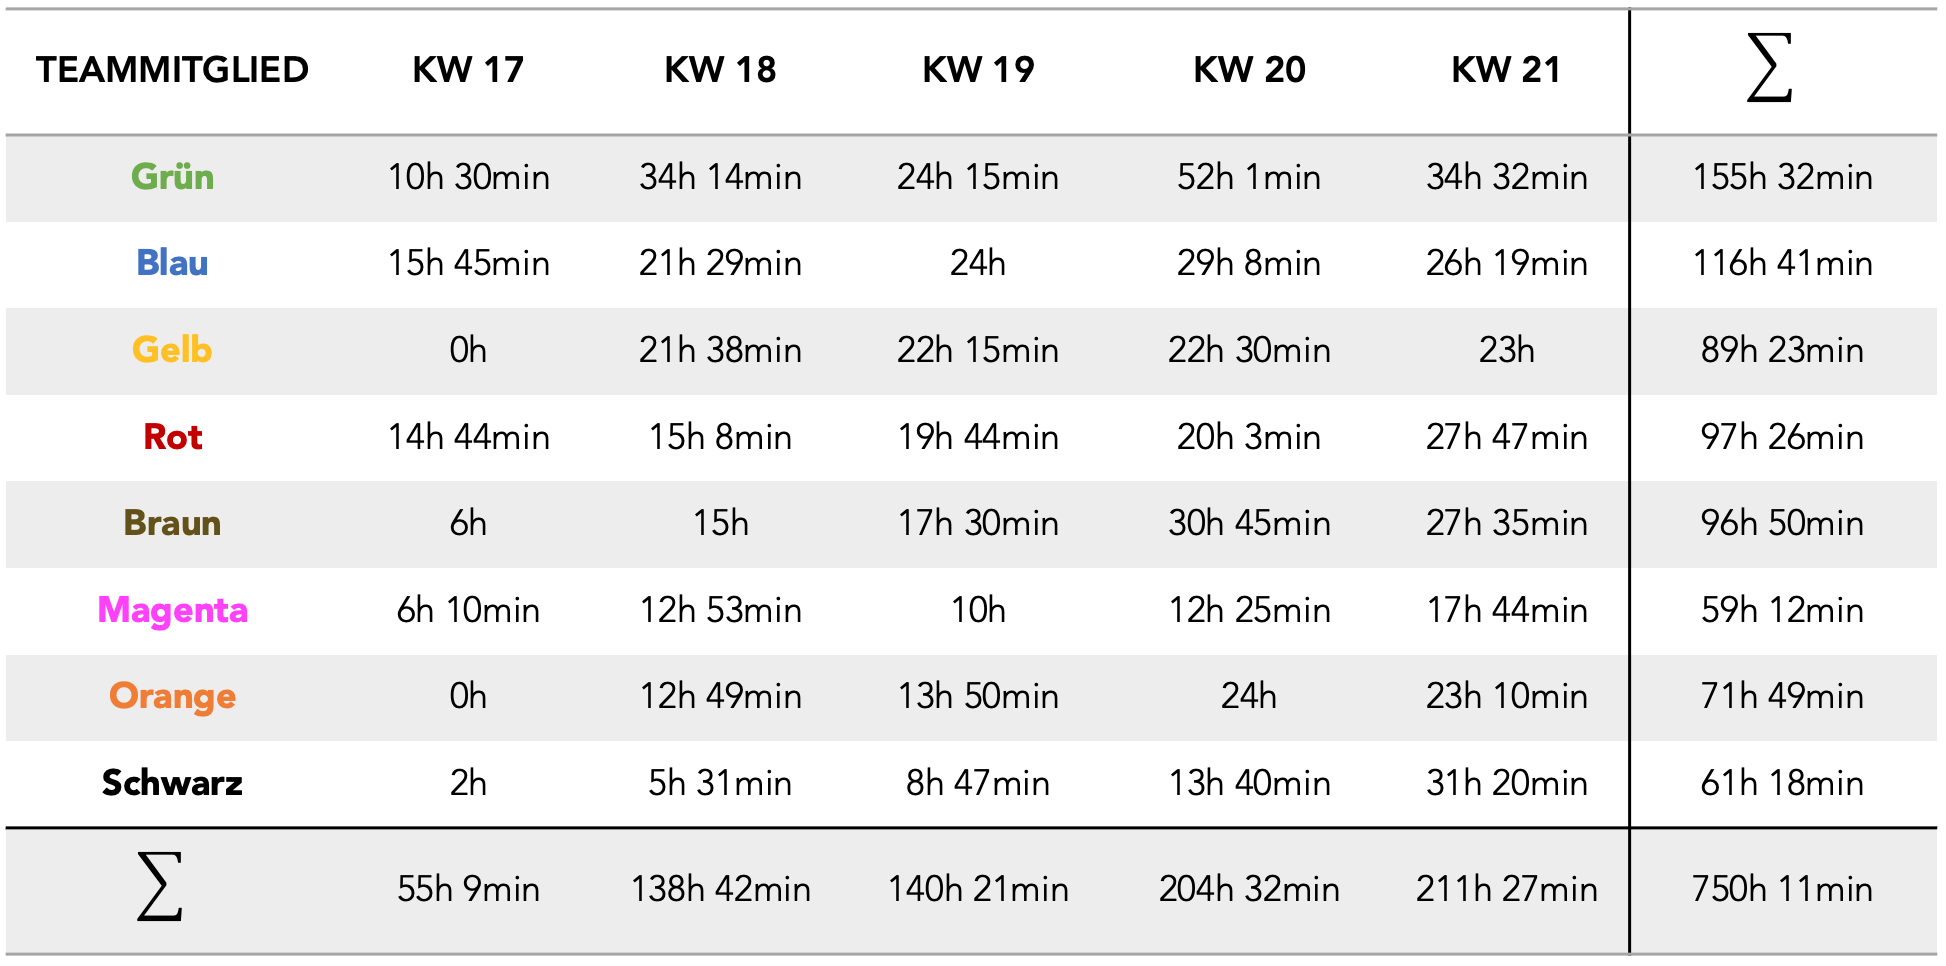
\includegraphics[width = \linewidth]{img/Kimai4.png}
    \caption{Planungs- und Entwurfsphase (KW 17-21): Tabelle zum Zeitaufwand der einzelnen Teammitglieder}
    \label{teammitglieder2}
\end{figure}

Den Abbildungen \ref{teammitglieder} und \ref{teammitglieder2} ist zu entnehmen, dass teilweise große Unterschiede zwischen den Teammitgliedern in Bezug auf die wöchentlich aufgebrachten Stunden für das Softwareprojekt bestehen. \footnote{\noindent Jede Linienfarbe in einem Projektmitglied zugeordnet. Auf die Beschriftung der einzelnen Linien wurde jedoch verzichtet, um die Anonymität der jeweiligen Personen zu wahren.}
Aus dem Diagramm geht hervor, dass in Kalenderwoche 17 noch nicht jeder seine Arbeitszeiten in das Kimai eingetragen hat, da es zu diesem Zeitpunkt Ihnen noch nicht zur Verfügung stand und sie diese hätten nachtragen müssen. Somit liegt bei zwei Personen der Wert in KW17 bei 0.
Es ist ein positiver Trend zu sehen, was auch in der Abbildung \ref{sollist} deutlich wurde.
Es ist hervorzuheben, dass einzelne Mitglieder weit über 20 Stunden pro Woche für das Softwareprojekt aufwenden. In der Kalenderwoche 20 liegt diese beispielsweise bei einem Teammitglied über 52 Stunden.


\section{Implementierungsphase}

Die folgenden Auswertungen wurden direkt nach Ende der Implementierungsphase vorgenommen.

\begin{figure} [h]
    \centering
    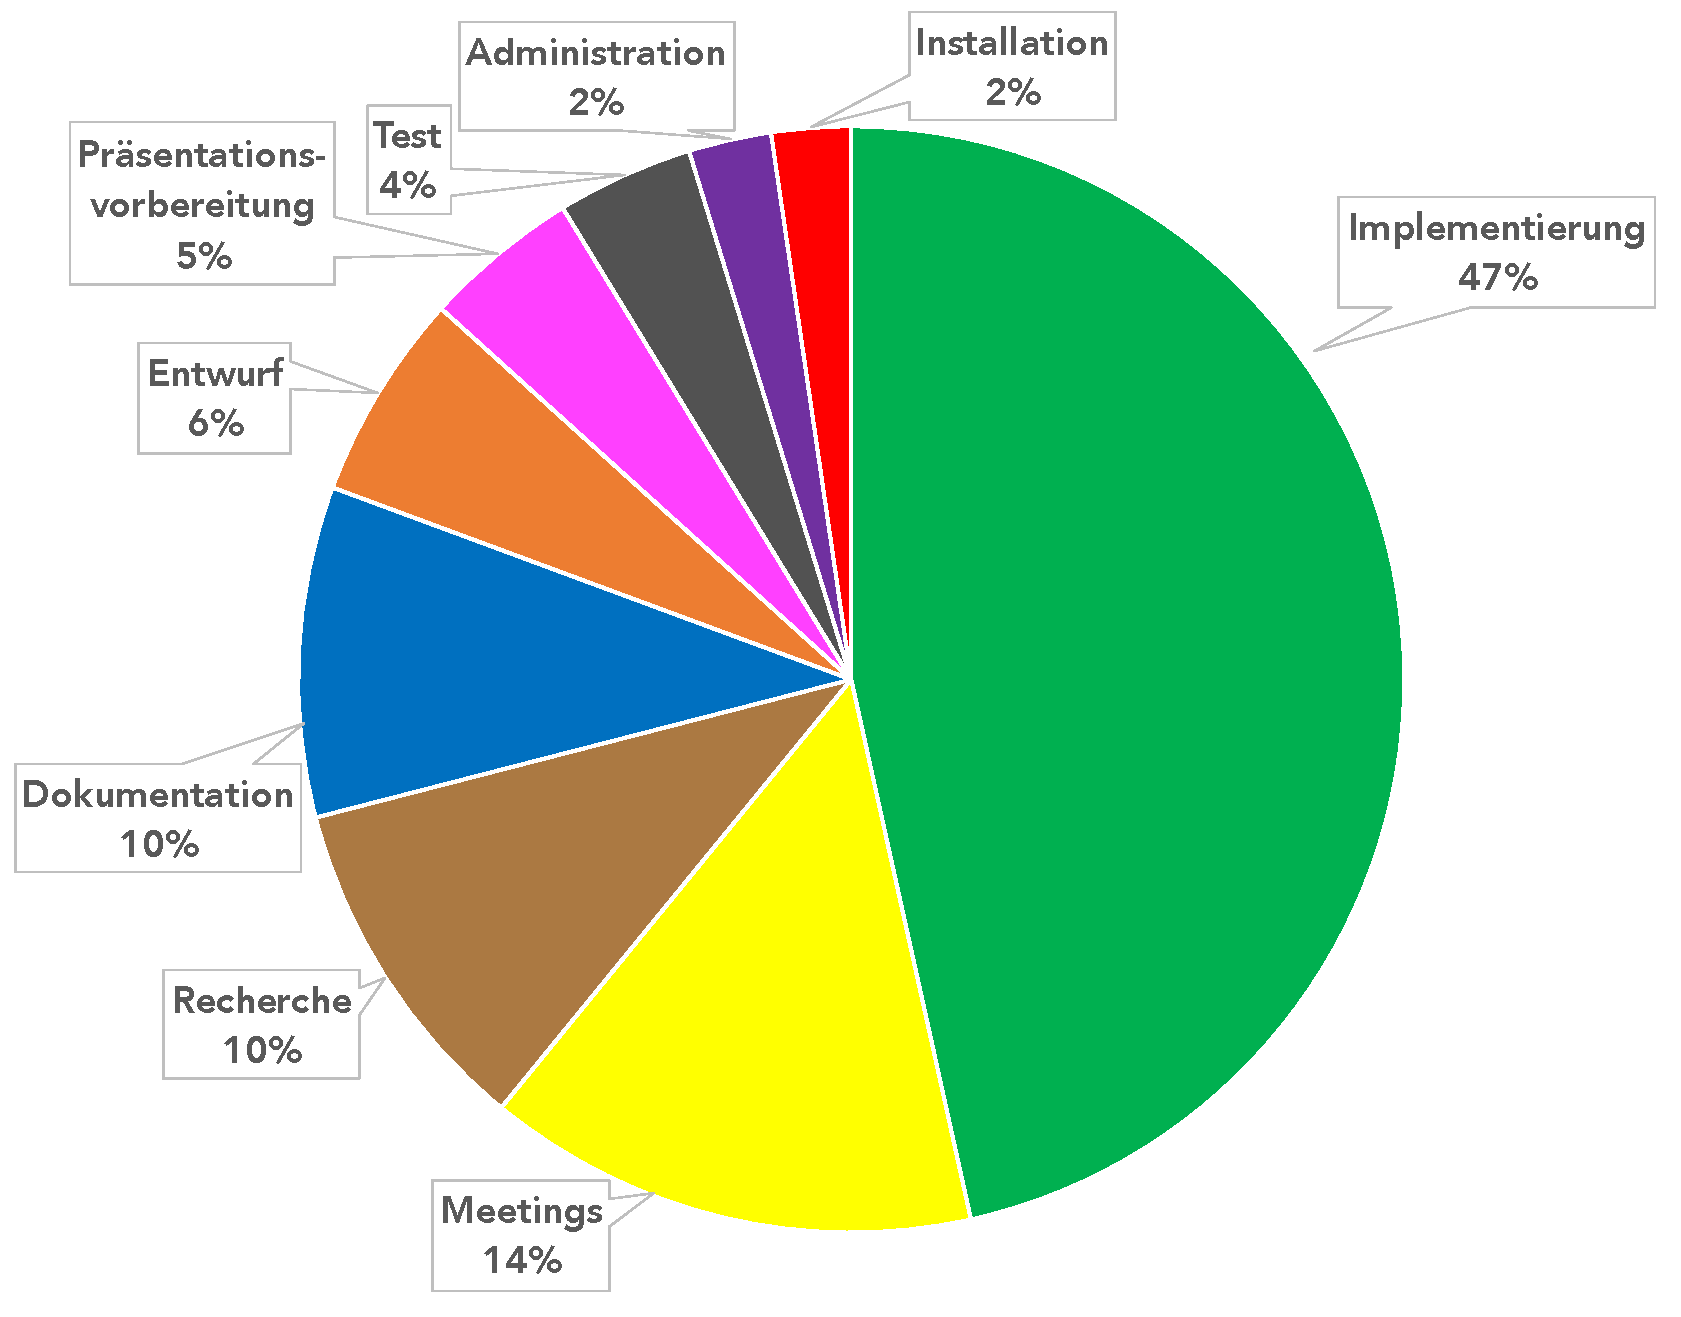
\includegraphics[width = 0.8\linewidth]{img/kimai5.pdf}
    \caption{Implementierungsphase (KW 22-24): Anteile der Aufgabenkategorien an der insgesamt aufgebrachten Zeit}
    \label{kimai5}
\end{figure}
Wie in Abbildung \ref{kimai5} zu sehen ist, wurde fast die Hälfte der Zeit dieser Projektphase für die \textbf{Implementierung} verwendet. Dieser Anteil ist durchaus angemessen, weil in der Implementierungsphase der größte Teil des Systems programmiert werden soll.

\textbf{Meetings} stellen mit 14\% die zweithäufigste Kategorie dar. Diese Größe bedarf nicht zwangsläufig einer Änderung, da die Meetings in dieser Phase lediglich wichtige Themen umfasst haben und so kurz wie möglich gehalten wurden. Außerdem bleibt zu erwähnen, dass in zwei Meetings ein Code-Review durchgeführt wurde, wodurch alle Teammitglieder voneinander lernen konnten und das System insgesamt sowie von anderen entwickelte Komponenten besser verstanden werden konnten.

Die Kategorien \textbf{Recherche} und \textbf{Dokumentation} nahmen beide ein Zehntel der insgesamt aufgebrachten Zeit in Anspruch und gehen somit mit einem angemessenen Anteil in das Projekt ein.

Die 6\%, die dem \textbf{Entwurf} zugeordnet werden können, sind relativ wenig. Möglicherweise wurde für diese Kategorie aufgebrachte Zeit auch in andere Kategorien wie Dokumentation oder Implementierung gebucht.

Positiv zu bewerten ist, dass die restlichen Kategorien, also \textbf{Präsentationsvorbereitung}, \textbf{Test}, \textbf{Administration} und \textbf{Installation}, höchstens 5\% der Zeit in Anspruch genommen haben. Trotzdem ist es wichtig, dass die den Tests zugeordnete Zeit in der kommenden Validierungsphase sprunghaft ansteigt. In der Implementierungsphase hat es sich dabei vor allem um Unit-Tests gehandelt, die für die gesamte Validierung nicht ausreichen werden.

\begin{figure} [h]
    \centering
    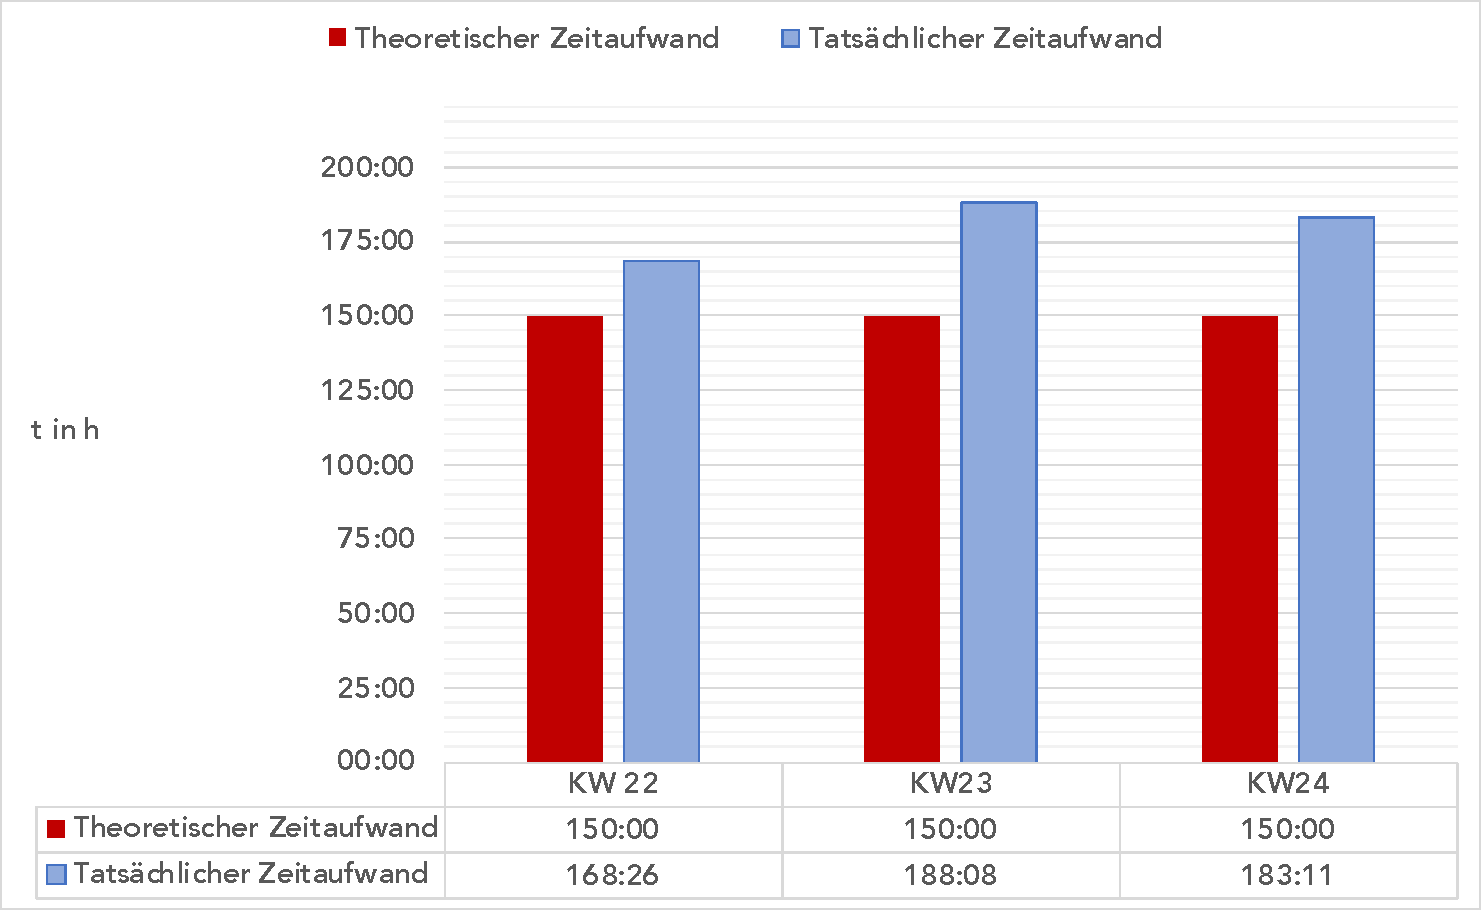
\includegraphics[width = \linewidth, trim=10pt 5pt 10pt 10pt, clip]{img/kimai7.pdf}
    \caption{Implementierungsphase (KW 22-24): Vergleich des theoretischen Aufwands mit dem tatsächlichen Aufwand}
    \label{kimai7}
\end{figure}
Abbildung \ref{kimai7} macht deutlich, dass in jeder einzelnen Woche der Implementierungsphase (KW 22 - 24) der tatsächliche Zeitaufwand über dem theoretischen Zeitaufwand lag. Die vorgegebenen 150 Stunden Zeitaufwand pro Woche wurden in der Kalenderwoche 23 sogar um über 38 Stunden überschritten. Wenn diese 38 Stunden durch die Anzahl der Teammitglieder geteilt wird, die bei acht liegt, wird deutlich, dass in dieser Woche im Durchschnitt jedes Teammitglied 4 Stunden und 45 Minuten mehr Zeit für das Softwareprojekt aufgewendet hat als vorgegeben.
\begin{figure} [h]
    \centering
    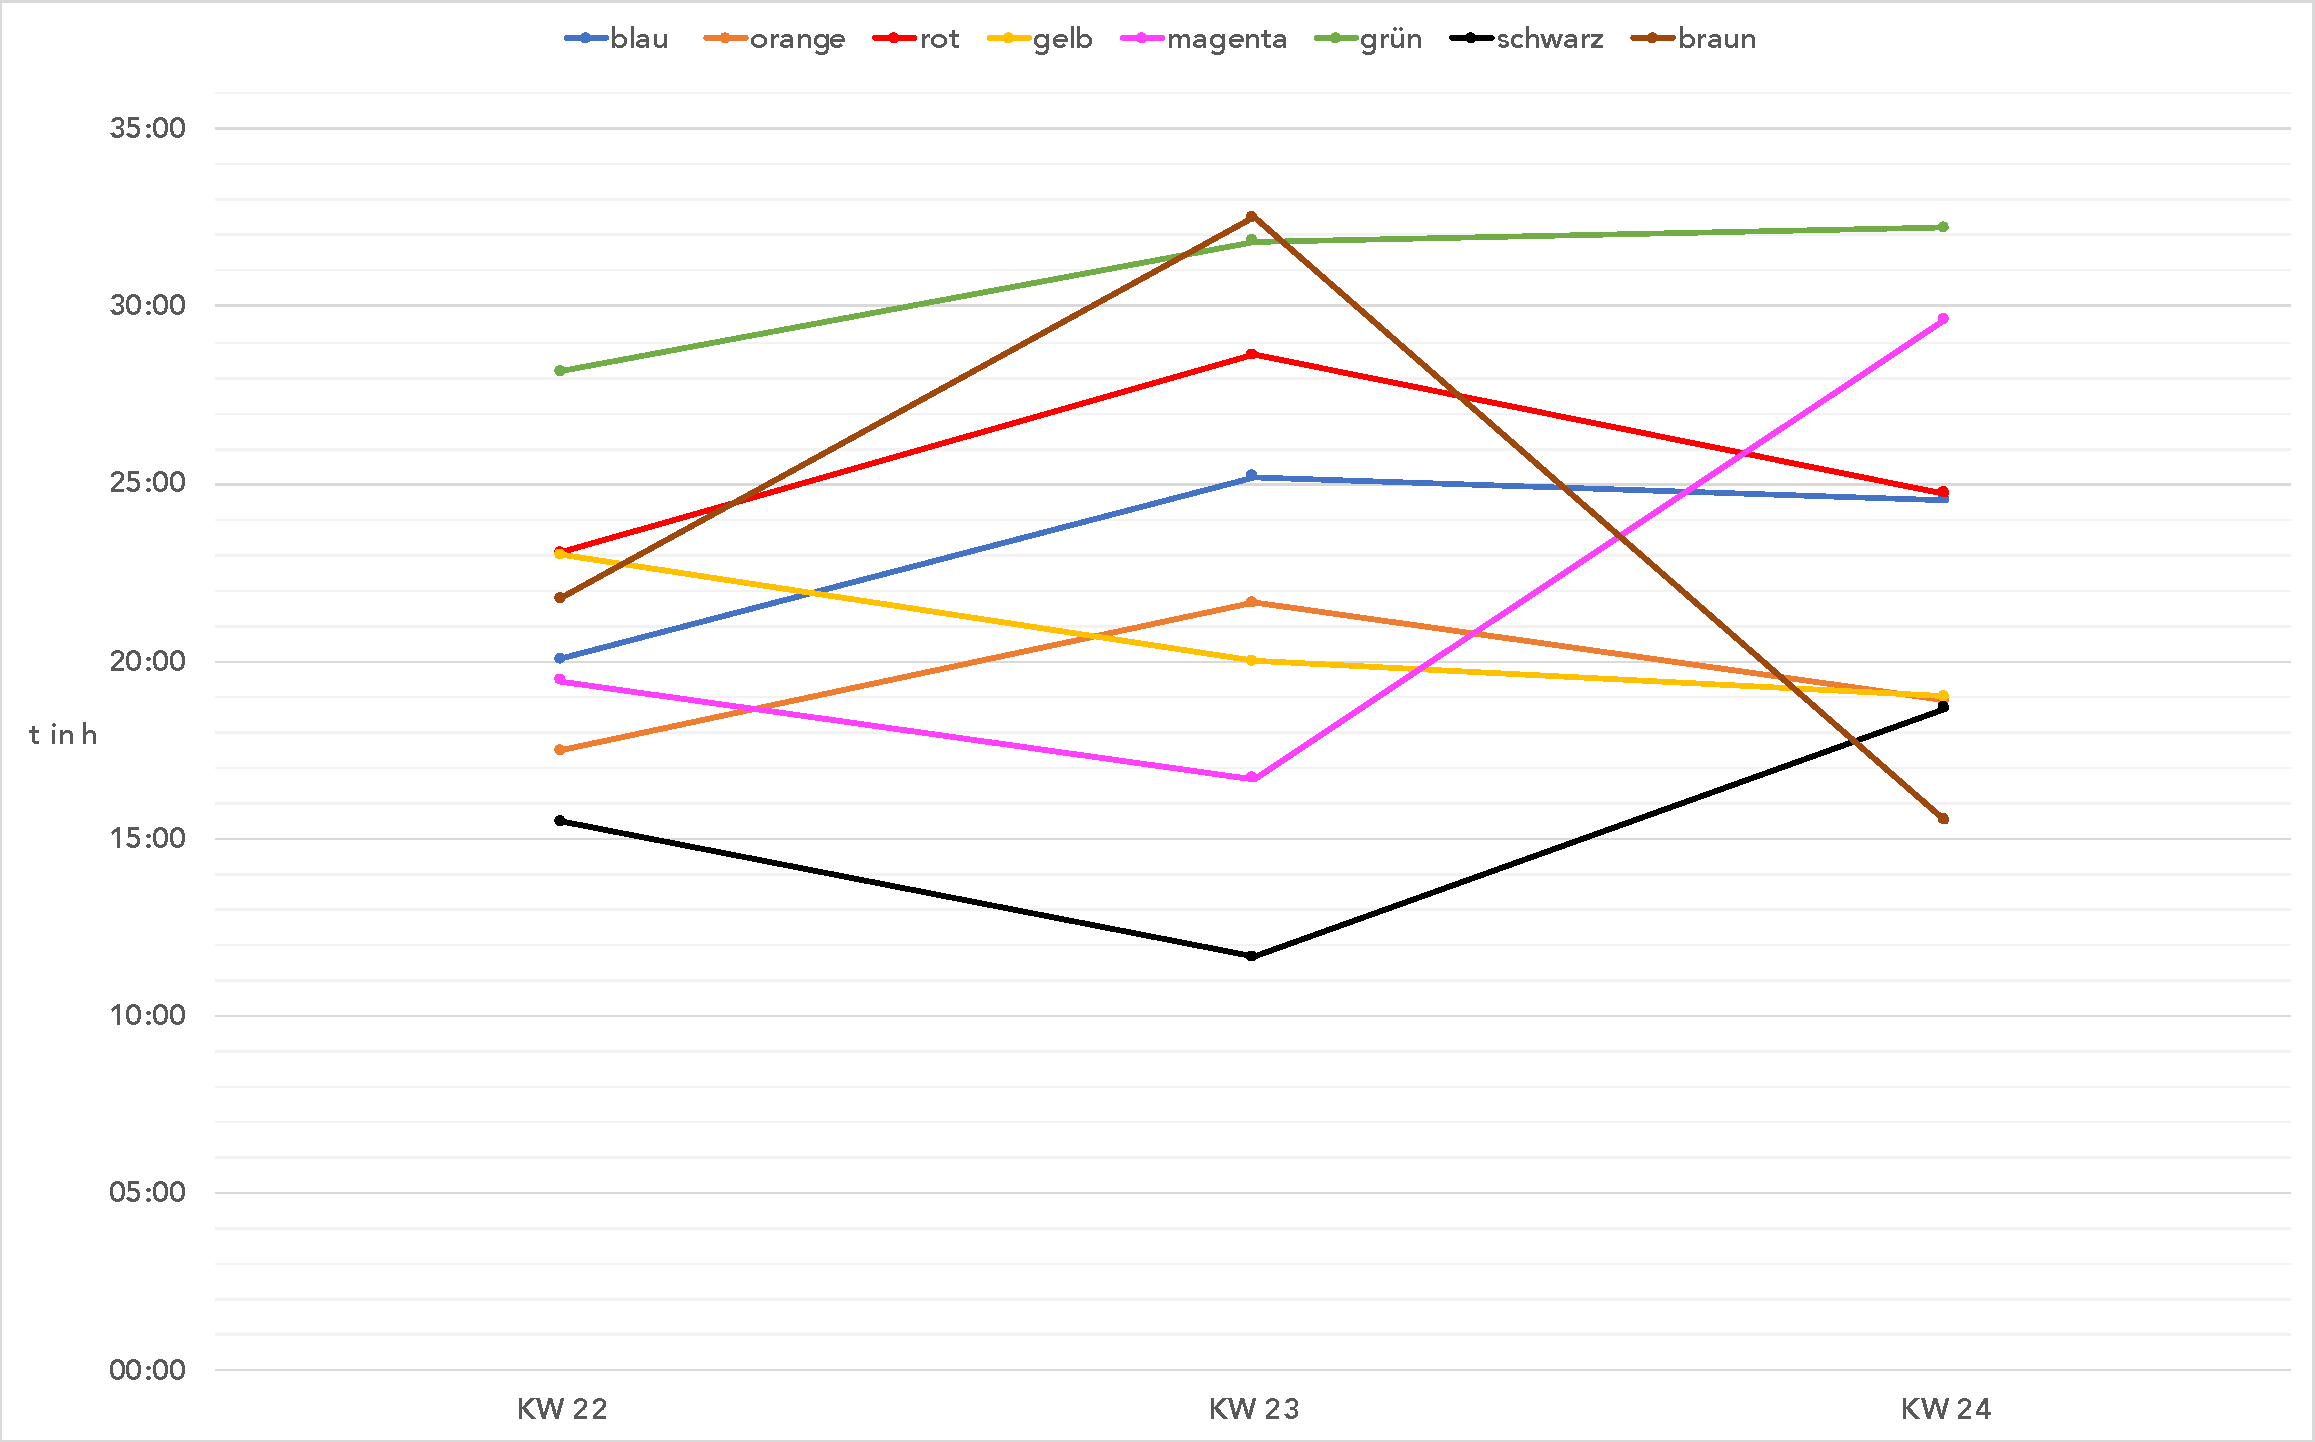
\includegraphics[width = \linewidth, trim=10pt 10pt 10pt 10pt, clip]{img/kimai9.pdf}
    \caption{Implementierungsphase (KW 22-24): Zeitaufwand der einzelnen Teammitglieder}
    \label{kimai9}
\end{figure}

Aus Abbildung \ref{kimai9} lässt sich grundsätzlich kein starker Anstieg der Zeit, die jeder einzelne Beteiligte für das Softwareprojekt aufgewendet hat, erkennen. Bei sechs der acht Teammitglieder liegt ihr persönliches Maximum in diesem Zeitraum in KW 23. Hier liegt auch der Punkt, mit dem größten Wert in der Implementierungsphase. Der dazugehörige Wert beträgt 32 Stunden und 30 Minuten (vgl. Abb. \ref{kimai11}).
Bei einigen Teammitglieder kann erkannt werden, dass die empfohlene Zeit von 15 bzw. 20 Stunden in einzelnen Fällen unterschritten wird. Üblicherweise wird auf die gesamte Zeit bezogen der Soll-Wert allerdings erfüllt, was auch in Abbildung \ref{kimai7} erkannt werden kann.

\begin{figure} [h]
    \centering
    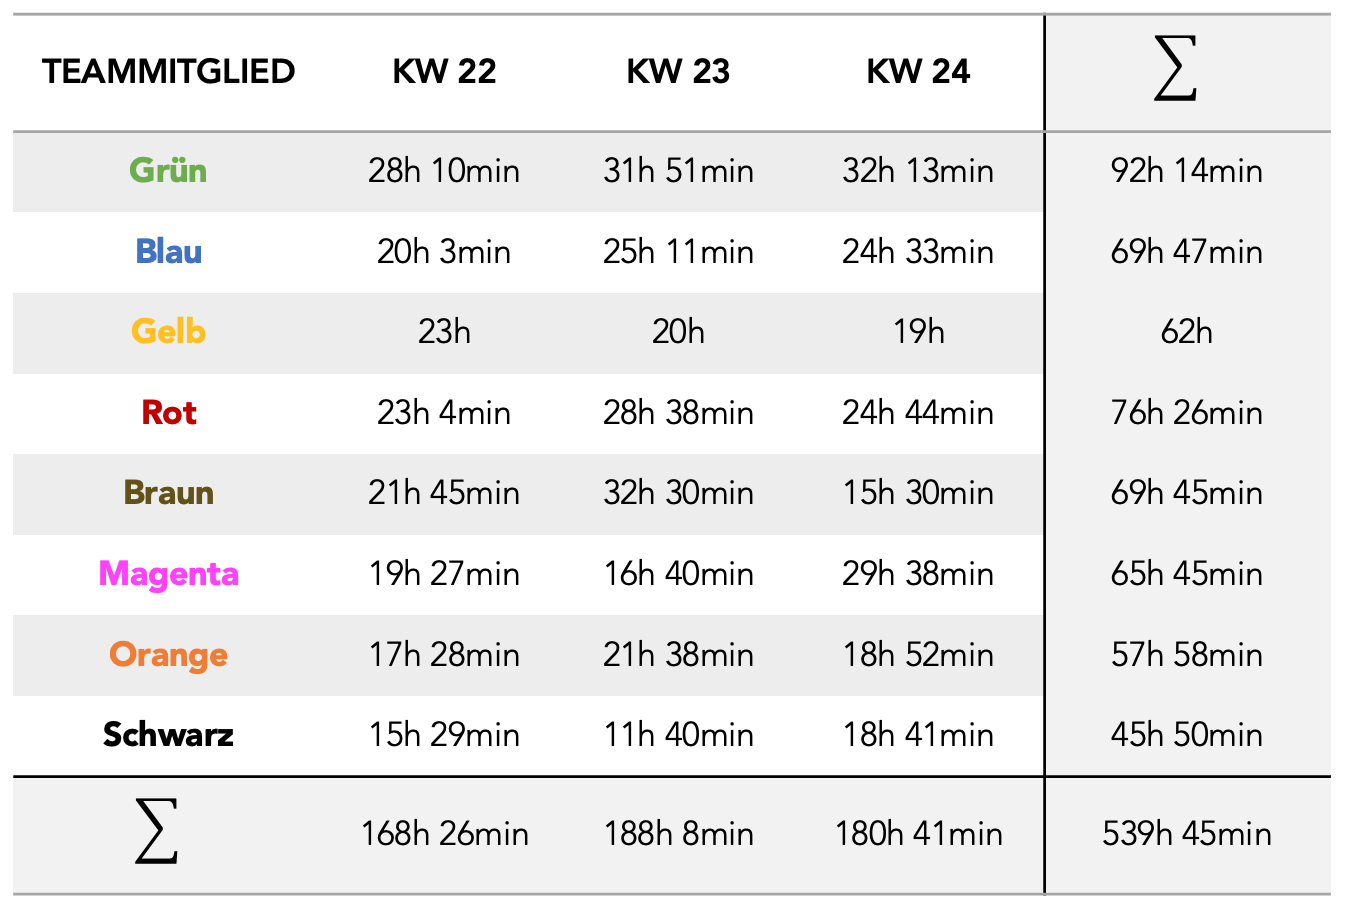
\includegraphics[width = 0.8\linewidth]{img/kimai11.png}
    \caption{Implementierungsphase (KW 22-24): Tabelle mit den erfassten Zeiten}
    \label{kimai11}
\end{figure}

\section{Validierungsphase}
\begin{figure} [h]
    \centering
    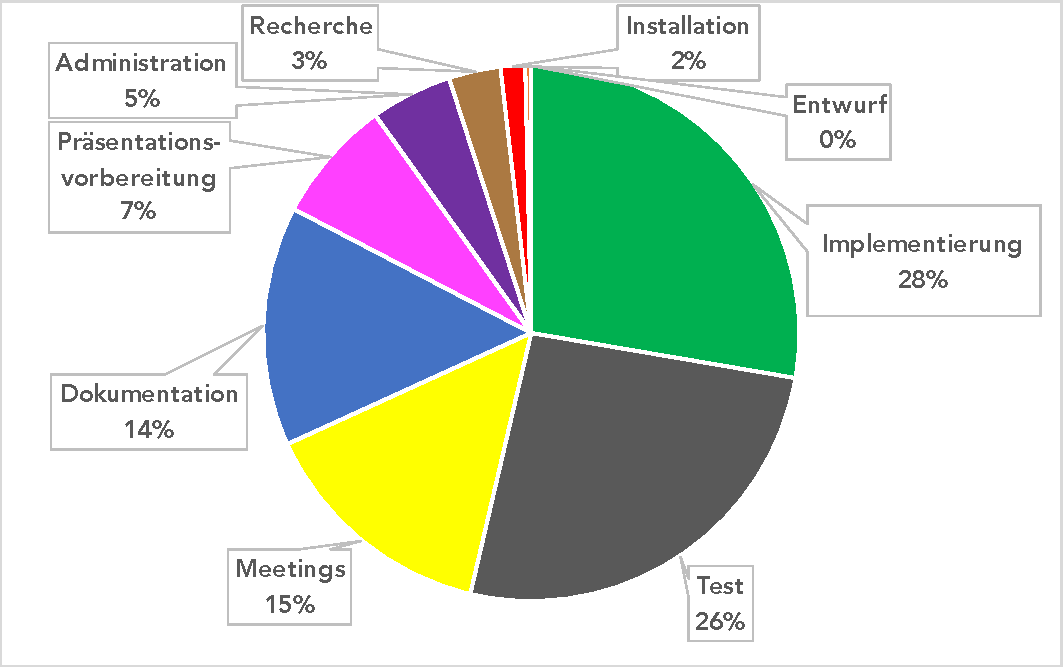
\includegraphics[width = 0.9\linewidth, trim=10pt 10pt 10pt 2pt, clip]{img/KreisVal.pdf}
    \caption{Validierungsphase (KW 25-28): Anteile der Aufgabenkategorien an der insgesamt aufgebrachten Zeit}
    \label{kimai19}
\end{figure}

In der Validierungsphase, also der letzten Phase des Softwareprojekts, wurden wieder Zeiten indie  ganz unterschiedlichen Kategorien gebucht. Die Verteilung kann im Diagramm in Abbildung \ref{kimai19} abgelesen werden.

Während für die \textbf{Implementierung} in der zweiten Phase des Projekts noch fast die Hälfte der Zeit aufgebracht wurde, hat sich dieser Wert in der Validierungsphase mit 28\% auf etwas mehr als ein Viertel reduziert. Das war auch zu erwarten, weil der größte Teil der eigentlichen Programmierung schon in dieser vorherigen Phase erledigt gewesen ist. Dennoch kann festgehalten werden, dass auch über die gesamte Phase noch implementiert wurde.

Nicht immer klar von der Implementierung abzugrenzen ist die Kategorie \textbf{Test}. So gehen diese beiden Kategorien teilweise ineinander über,das heißt, beide Tätigkeiten wurden des Öfteren zusammen erledigt. Deshalb kann eine gewisse Ungenauigkeit bzw. Verschmelzung der beiden Anteile nicht ausgeschlossen werden. Etwas mehr als ein Viertel der Gesamtzeit, genauer gesagt 26\%, wurde für das Testen gebucht. Vor Beginn der Phase hätte vermutet werden können, dass dieser Wert höher ausfällt. Das Nichteintreten dieser Vermutung könnte aus der Überschneidung mit der Kategorie Implementierung und aus dem relativ hohen Zeitaufwand für andere Kategorien resultieren.

Während die \textbf{Meetings} in den vergangenen beiden Phasen an erster und zweiter Stelle standen, sind diese in der Validierungsphase erstmals an dritter Stelle zu finden, und zwar mit einem Anteil von 15\%. Beim Vergleich dieses Wertes mit der ersten Phase fällt auf, dass gegen Ende des Projekts nur noch ca. halb so viel Zeit mit Meetings verbracht wurde wie am Anfang, was positiv zu bewerten ist. Es mussten allerdings auch wesentlich weniger grundlegende Entscheidungen über das Projekt diskutiert und entschieden werden. Das am Montag Abend stattfindende Meeting dauerte fast immer am längsten, unter anderem deshalb, weil Martin Backhaus in dieser Zeit Feedback zum geschriebenen Code gab und wichtige Verbesserungen besprochen wurden. Die restlichen wöchentlichen Meetings fielen dann meist wesentlich kürzer aus und wurden meist für kurze Statusabfragen und für die Klärung individueller Fragen genutzt.

14\% der Zeit wurde für die \textbf{Dokumentation} verwendet. Diese hat in der Validierungsphase etwas weniger Zeit in Anspruch genommen als vermutet, womöglich weil sich lediglich einige wenige Teammitglieder besonders viel mit der Dokumentation beschäftigt haben. Die Mehrheit des Teams hat sich gegen Ende des Projekts tendentiell eher für andere Aufgaben verantwortlich gefühlt, was allerdings kein Problem darstellte.

Die \textbf{Präsentationsvorbereitung} muss hier an nächster Stelle angemerkt werden, denn ihr ist ein Wert von 7\% zuzuordnen. Die Abschlusspräsentation findet in dieser Phase erstmals in Präsenz im Audimax der TU Ilmenau statt und bedarf daher einer besonderen Vorbereitung. Die möglichst gut zu erkennende Darstellung der Funktionalität des Systems steht hierbei an erster Stelle. Für diese visuelle Darstellung wurde ein kurzes PyQT-Programm geschrieben.

Die \textbf{Administration} nahm 5\% der Zeit in Anspruch. Eine wichtige administrative Aufgabe dieser Phase war zum Beispiel das Erstellen und Auswerten der durchgeführten Umfrage, deren Ergebnisse im 9. Kapitel dieses Dokuments zu finden sind.

Die verbleibenden Kategorien \textbf{Recherche} (3\%), \textbf{Installation} (2\%) und \textbf{Entwurf} (<0,5\%) wurden in der letzten Projektphase kaum gebucht. Das lässt sich damit begründen, dass es sich bei diesen um typische Aufgaben des Projektbeginns handelt.

\begin{figure} [h]
    \centering
    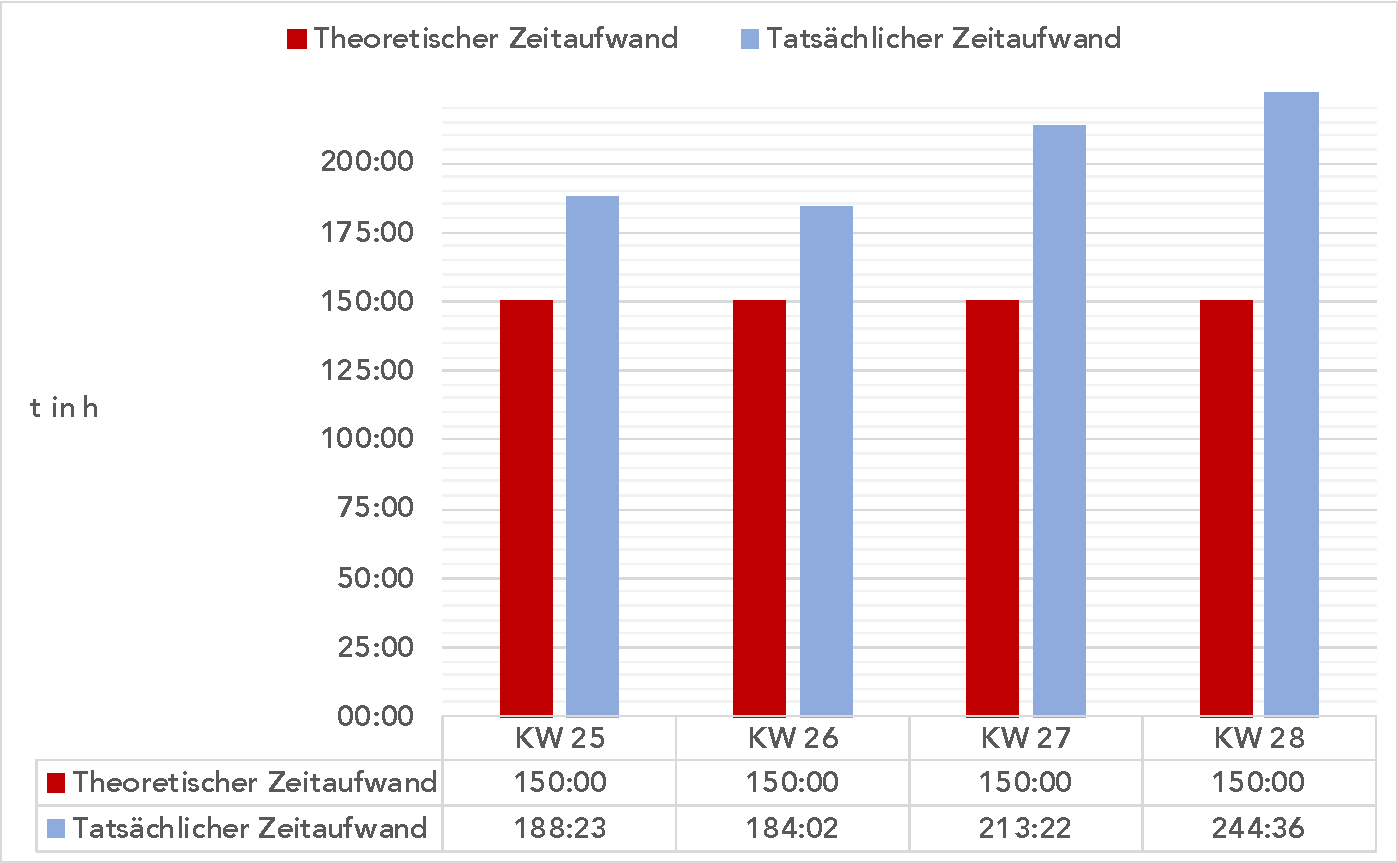
\includegraphics[width = \linewidth, trim=5pt 5pt 5pt 5pt, clip]{img/phase3.pdf}
    \caption{Validierungsphase (KW 25-28): Vergleich des theoretischen Aufwands mit dem tatsächlichen Aufwand}
    \label{kimai14}
\end{figure}

Aus der Abbildung \ref{kimai14} wird ersichtlich, dass das Ziel von 150 Wochenstunden in allen Wochen dieser Projektphase (KW 25-28) erreicht wurde. Es bleibt erneut anzumerken, dass auch während der ersten drei Tage der KW 29 noch am Softwareprojekt gearbeitet wird. Sollte das Reviewdokument diese Zeiten auch noch enthalten, könnte es erst nach Ende des Projekts fertig gestellt werden. Es muss allerdings noch vor dem letzten Review abgegeben werden. Der erfasste Aufwand überstieg den theoretischen in allen Wochen sogar um über 30 Stunden. Die tatsächlich insgesamt aufgebrachten Zeit kann also durchaus als zufriedenstellend bezeichnet werden.

\begin{figure} [h]
    \centering
    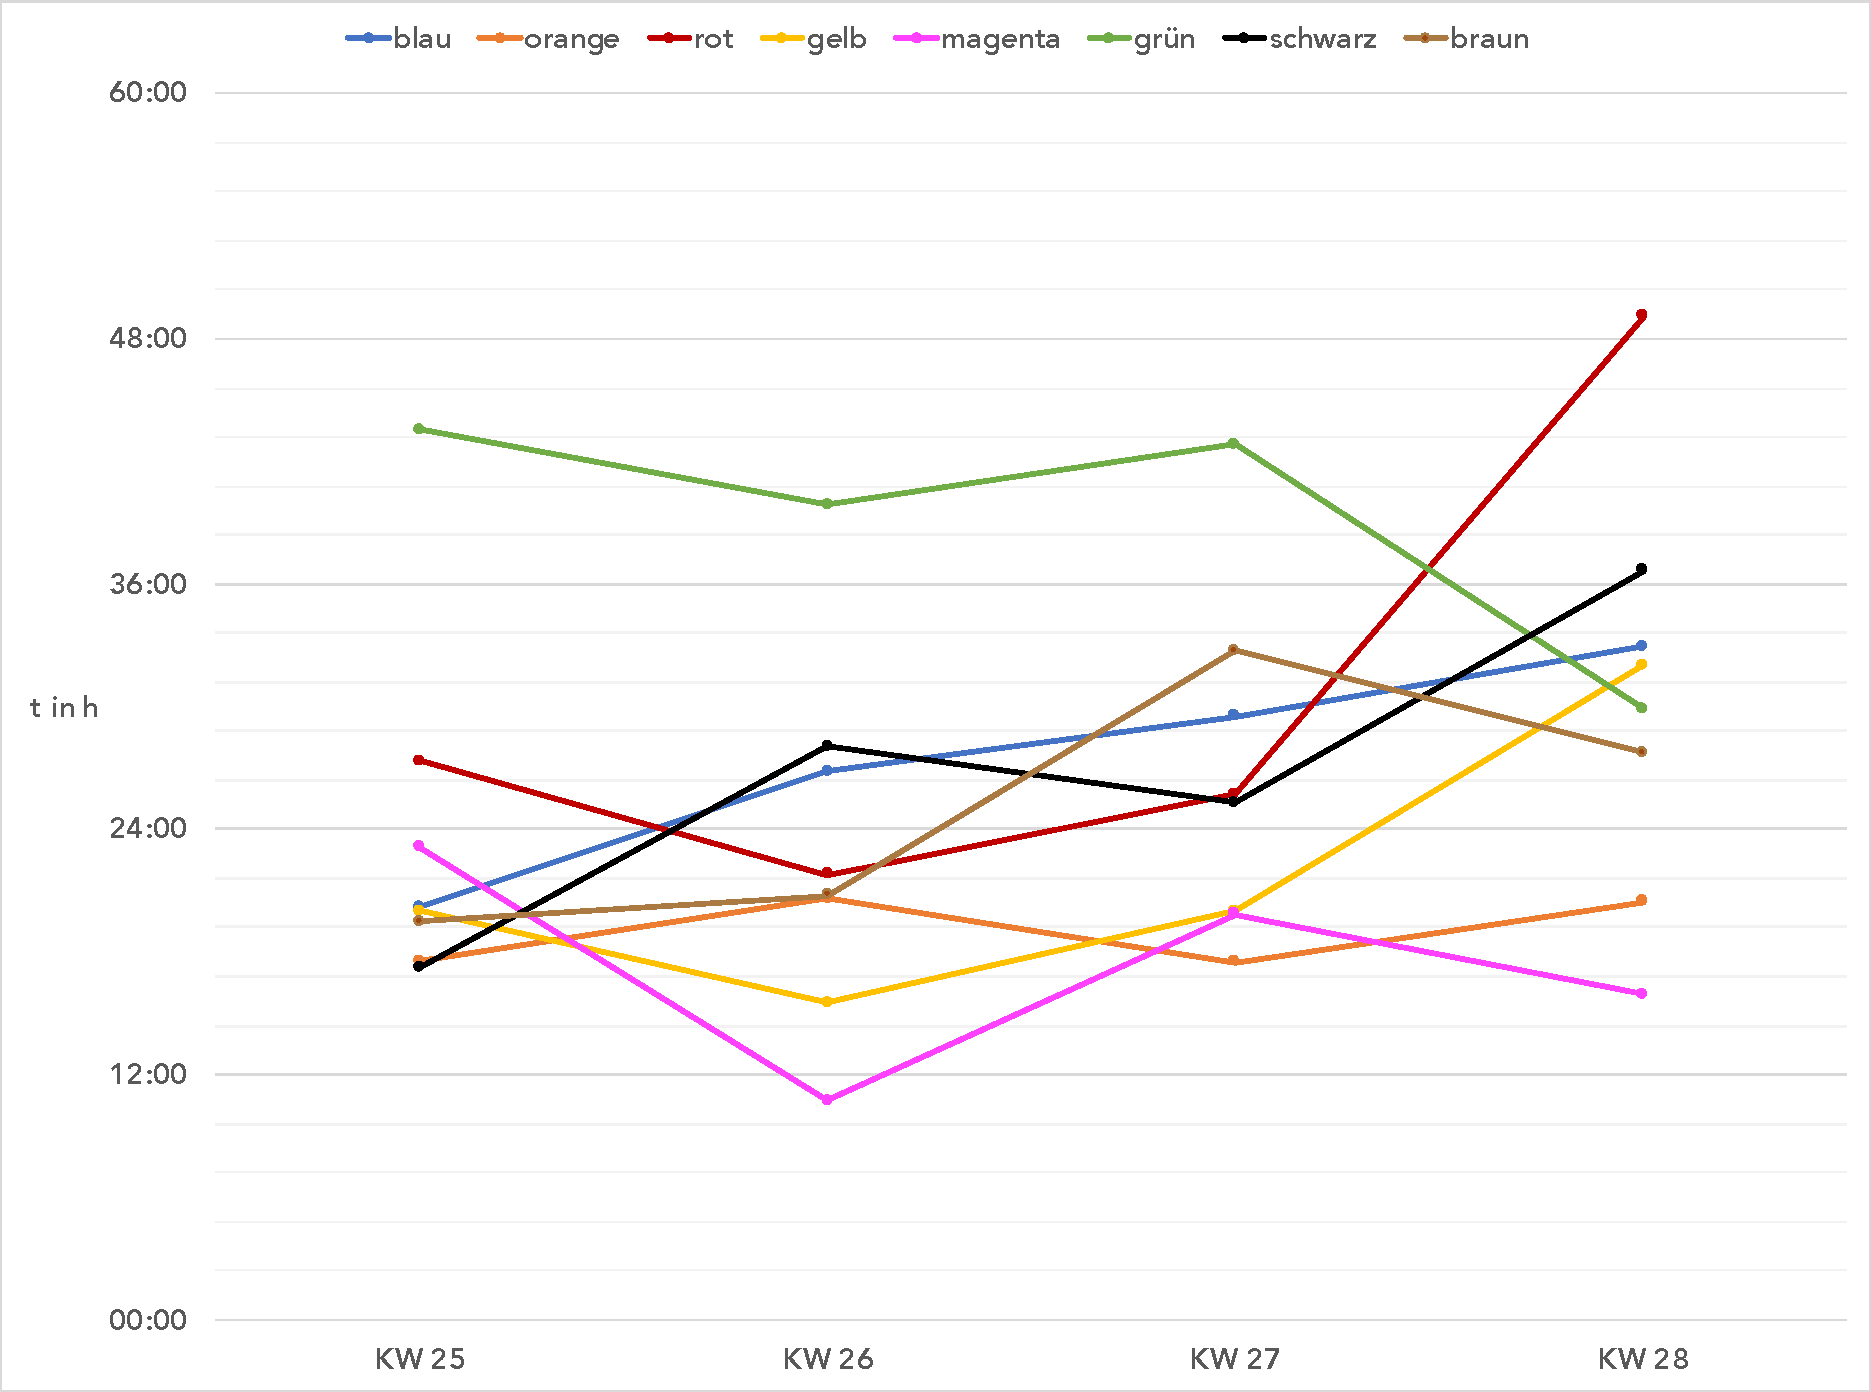
\includegraphics[width = \linewidth, trim=5pt 5pt 5pt 5pt, clip]{img/zeiten2.pdf}
    \caption{Validierungsphase (KW 25-28): Zeitaufwand der einzelnen Teammitglieder}
    \label{kimai13}
\end{figure}

Die Unterschiede zwischen den einzelnen Teammitgliedern können aus Abbildung \ref{kimai13} abgelesen werden. Die längste Wochenarbeitsdauer wurde mit 43:31 h in KW 25 erreicht. Ein Teammitglied konnte krankheitsbedingt in KW 26 nur weniger als 11 Stunden mit dem Softwareprojekt beschäftigt sein (vgl. Abb. \ref{kimai20}). Auch in dieser Phase kann wieder erkannt werden, dass der Plan-Wert in Einzelfällen unterschritten wurde. Diese Defizite wurden in den allermeisten Fällen dann allerdings in anderen Wochen aufgeholt.

\begin{figure} [h]
    \centering
    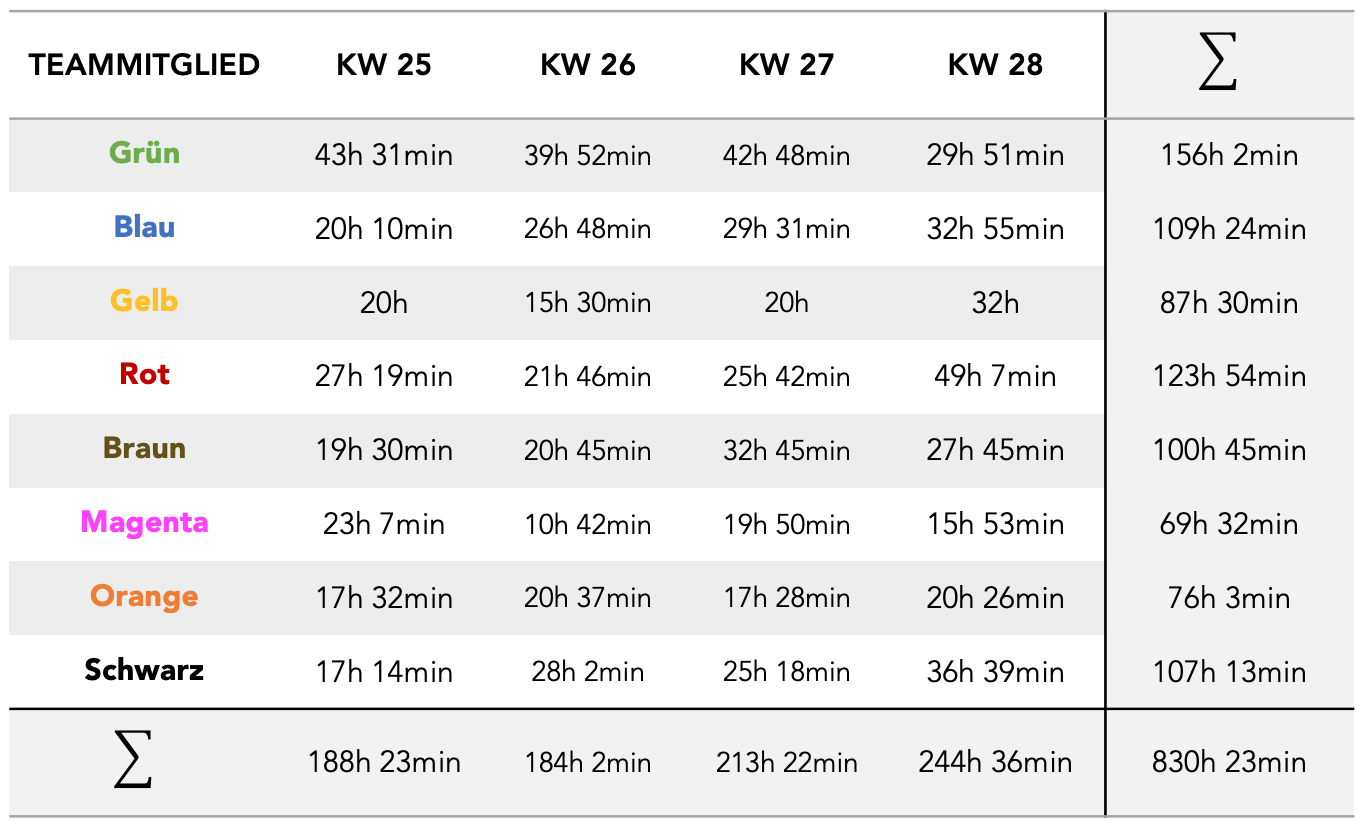
\includegraphics[width = 0.8\linewidth]{img/tabelle1.png}
    \caption{Validierungsphase (KW 25-28): Tabelle mit den erfassten Zeiten}
    \label{kimai20}
\end{figure}

\section{Vergleich der Planungs- und Entwurfsphase mit der Implementierungsphase}

Dieses Kapitel wurde gegen Ende der Implementierungsphase erstellt.

\begin{figure} [h]
    \centering
    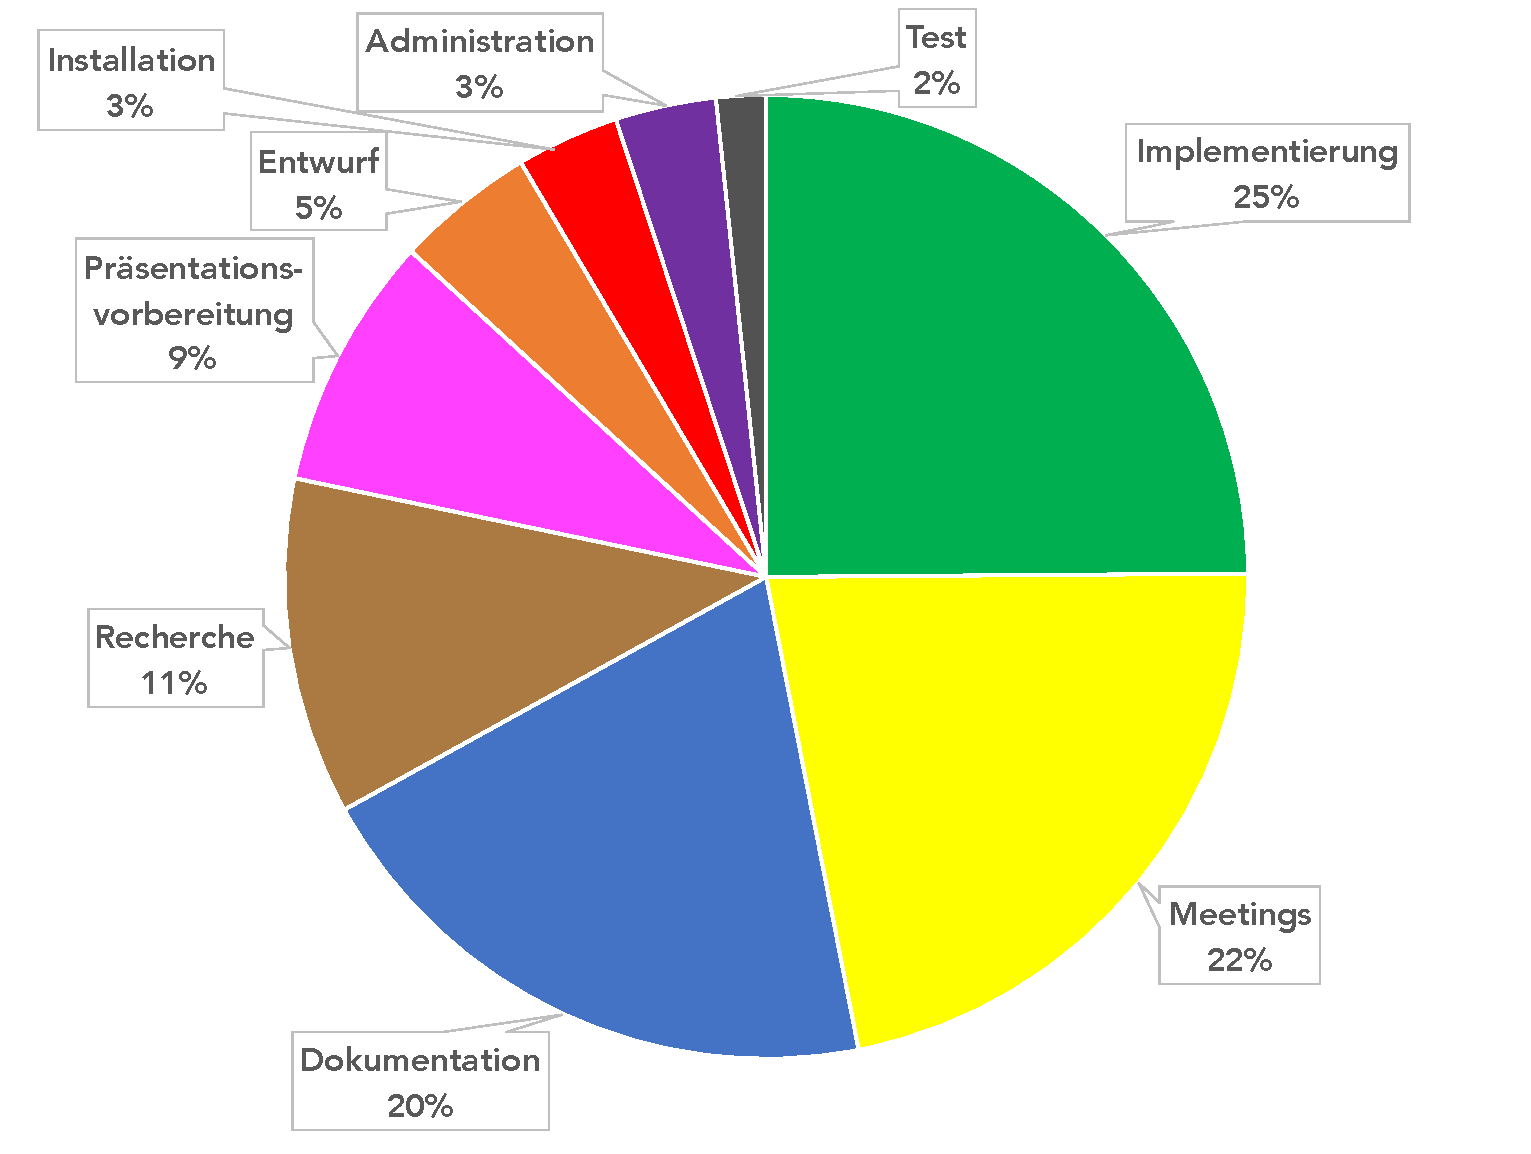
\includegraphics[width = 0.9\linewidth]{img/kimai6.pdf}
    \caption{Planungs- und Entwurfsphase und Implementierungsphase (KW 17-24): Anteile der Aufgabenkategorien an der insgesamt aufgebrachten Zeit}
    \label{kimai6}
\end{figure}
In Abbildung \ref{kimai7} wird die Verteilung der Kategorien bezogen auf den gesamten Projektzeitraum, d. h. in diesem Fall die ersten beiden Phasen, dargestellt.

Bei einem Vergleich der Anteile der Kategorien an der insgesamt aufgebrachten Zeit zwischen Planungs- und Entwurfsphase und Implementierungsphase fällt als erstes auf, dass sich die für die \textbf{Implementierung} aufgebrachte Zeit vervielfacht hat. Dieser sprunghafte Anstieg wurde auch prognostiziert, weil die Implementierung in der ersten Phase lediglich einen ersten Prototyp umfasste und der zentrale Bestandteil der jetzt abgeschlossenen Phase ist.

Weiterhin ist der Anteil der \textbf{Meetings} von 29 auf 14\% gesunken. Da dieser Anteil im ersten Abschnitt des Softwareprojekts viel zu hoch war und schließlich auf einen adäquaten Wert gesenkt werden konnte, kann geschlussfolgert werden, dass die richtigen Maßnahmen getroffen wurden. So wurden Diskussionen, die nicht alle Teammitglieder betroffen haben, von den wöchentlichen Treffen in kleinere Gruppen verlagert und dann in der entsprechenden Kategorie themenbezogen gebucht.

Die \textbf{Dokumentation} hat während der Implementierungsphase ebenfalls weniger Zeit in Anspruch genommen als in der Planungs- und Entwurfsphase. Das umfassende Reviewdokument der ersten Phase, bestehend aus dem Pflichtenheft und einer Entwurfsdokumentation, stellte im ersten Monat des Projekts eine der Hauptaufgaben dar, während ihm in dieser Phase lediglich eine mittelhohe Priorität zugeordnet wurde.

Der \textbf{Rechercheaufwand} ist leicht gesunken, da sich zu Beginn des Projekts besonders viel Wissen angeeignet werden musste, welches im Laufe des Projekts dann zunehmen angewendet werden musste. Da fast alle Teammitglieder zu Beginn des Projekts recht unerfahren waren, scheinen die 11\% der im gesamten Projektzeitraum aufgebrachten Zeit ein geeigneter Anteil zu sein.

Insgesamt wurden 9\% der Zeit für die Vorbereitung von \textbf{Präsentationen} verwendet, was ebenfalls positiv zu bewerten ist. An dieser Stelle muss angemerkt werden, dass die Zeiterfassung der Implementierungsphase lediglich die Zeiten bis KW 24 umfasst, wodurch die letzten drei Tage vor der Präsentation nicht abgedeckt wurden. In dieser Zeit wird vermutlich noch eine nicht zu vernachlässigende Menge an Zeit für die Vorbereitung des zweiten Reviews investiert werden. Aus diesem Grund und weil jedes Teammitglied in der ersten Woche des Projekts eine Präsentation zu einem bestimmten Thema ausgearbeitet hat, ist der Wert von 11\% auf 5\% zurückgegangen.

Der \textbf{Entwurf} umfasste insgesamt 5\% der Zeit und wurde in beiden Phasen tendenziell zu wenig beziehungsweise in anderen, ähnlichen Kategorien erfasst.

Für die \textbf{Installation} musste sogar in der ersten Phase nur 5\% der Zeit verwendet werden. In der Implementierungsphase sank dieser Anteil auf 2\%. Da fast alle benötigten Komponenten bereits installiert sein sollten, lässt sich vermuten, dass der Anteil dieser Kategorie in der letzten Projektphase weiter gegen null geht.

Der \textbf{Administrationsaufwand} konnte schon in der ersten Phase des Projekts gering gehalten werden und ging auch in der Implementierungsphase in einem geeigneten Maß ein.

In der zweiten Phase hat sich der \textbf{Testaufwand} von 2 auf 4\% verdoppelt. Das zeigt, dass die Projektverlauf zunehmende Bedeutung des Testens erkannt wurde. Wichtig ist allerdings, dass beim Testen in der nächsten Phase ein sprunghafter Anstieg ähnlich wie bei der Implementierung zwischen erster und zweiter Phase zu erkennen ist.

\begin{figure} [h]
    \centering
    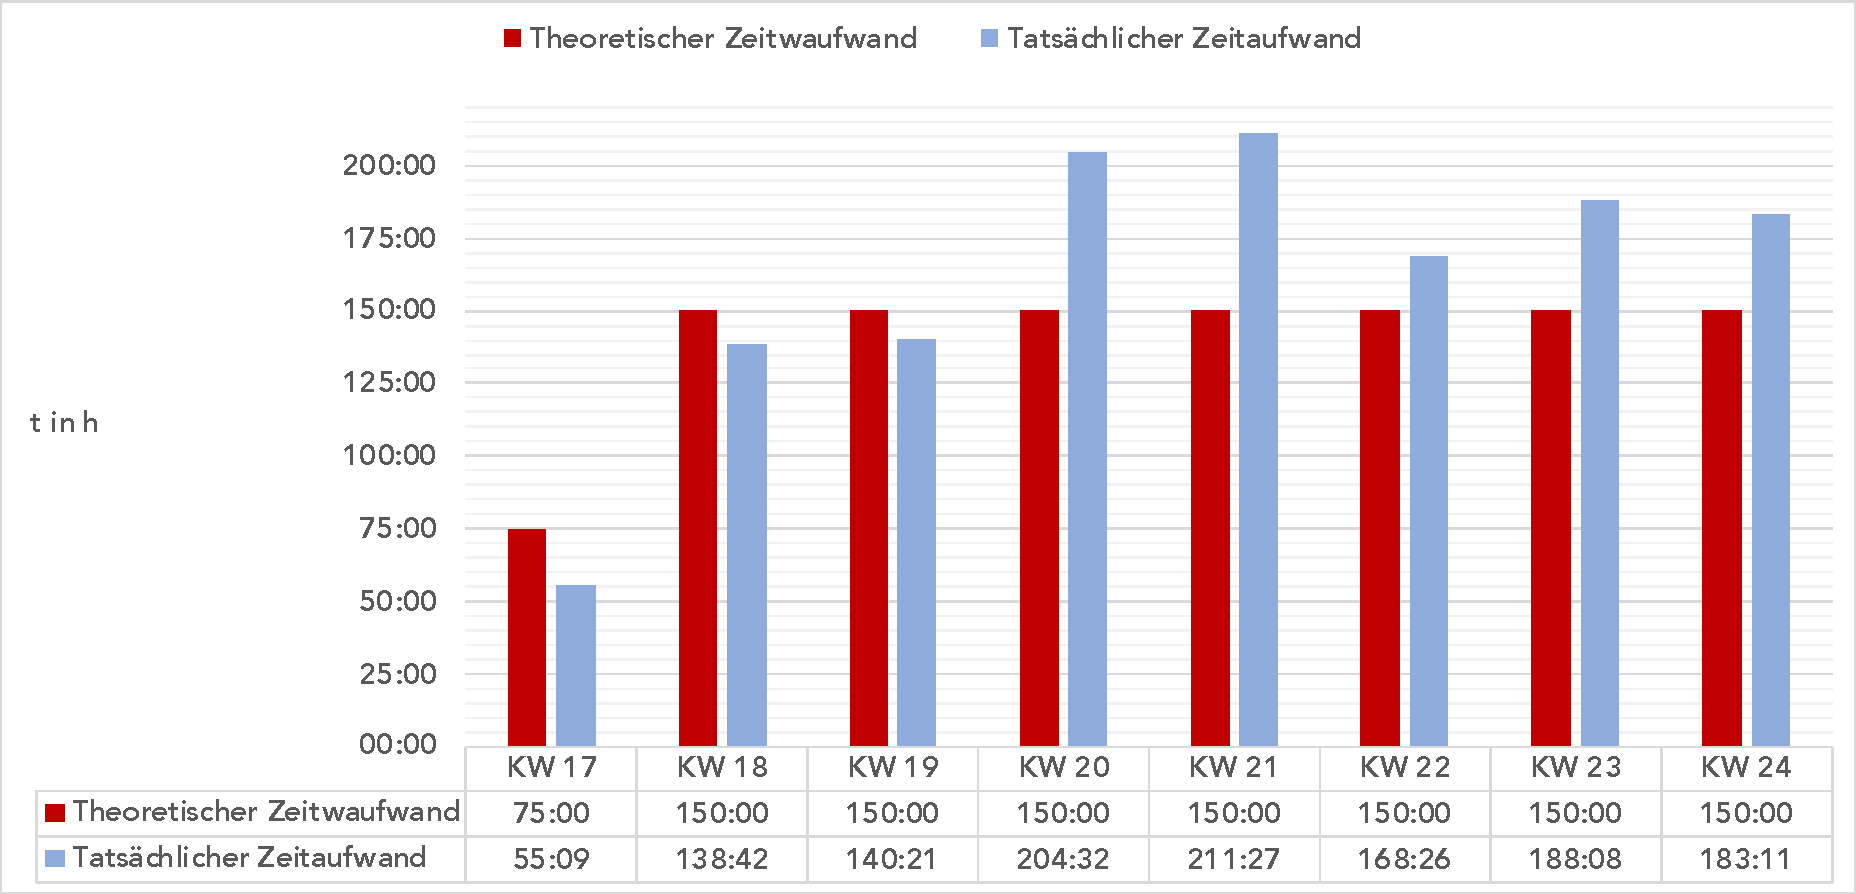
\includegraphics[width = \linewidth, trim=8pt 5pt 8pt 8pt, clip]{img/kimai8.pdf}
    \caption{Planungs- und Entwurfsphase und Implementierungsphase (KW 17-24): Vergleich des theoretischen Aufwands mit dem tatsächlichen Aufwand}
    \label{kimai8}
\end{figure}
Folgendes lässt sich in Abbildung \ref{kimai8} erkennen:
Während in den ersten drei Wochen des Softwareprojekts (KW 17-18) der tatsächliche Zeitaufwand noch leicht unter dem theoretischen Wert liegt, ändert sich dies in den darauffolgenden Wochen dahingehend, dass der tatsächliche Zeitaufwand den theoretischen (zum Teil stark) übersteigt.
Die Feststellung, dass mehr Zeit aufgewendet wird bzw. werden muss als vorgegeben,  stimmt mit der Aufwandsschätzung aus dem ersten Reviewdokument überein.
Denn wenn die theoretischen Werte aller bisherigen Wochen (KW 17-24) aufaddiert werden, ergibt sich ein Wert von 1289 Stunden und 56 Minuten (vgl. Abb. \ref{kimai12}). Diesem stehen 1125 Stunden entgegen:
\begin{align*}
    1 \cdot 75h+7 \cdot 150h= 1125h
\end{align*}
In der ersten Aufwandsschätzung schätzten wir den Aufwand des gesamten Projekts auf 2107 Stunden.
Würden wir in den kommenden Wochen (KW 25-29) \glqq lediglich\grqq{} den theoretische berechnete Zeit brauchen, wären das zu den bisher benötigten 1289 Stunden und 56 Minuten noch 675 Stunden, also insgesamt 1964 Stunden und 56 Minuten. Dieser Wert kommt dem Schätzwert aus der Aufwandsschätzung sehr nahe.
\begin {align*}
4 \cdot 150h + 1 \cdot 75h = 675h
\end{align*}

\begin{figure} [h]
    \centering
    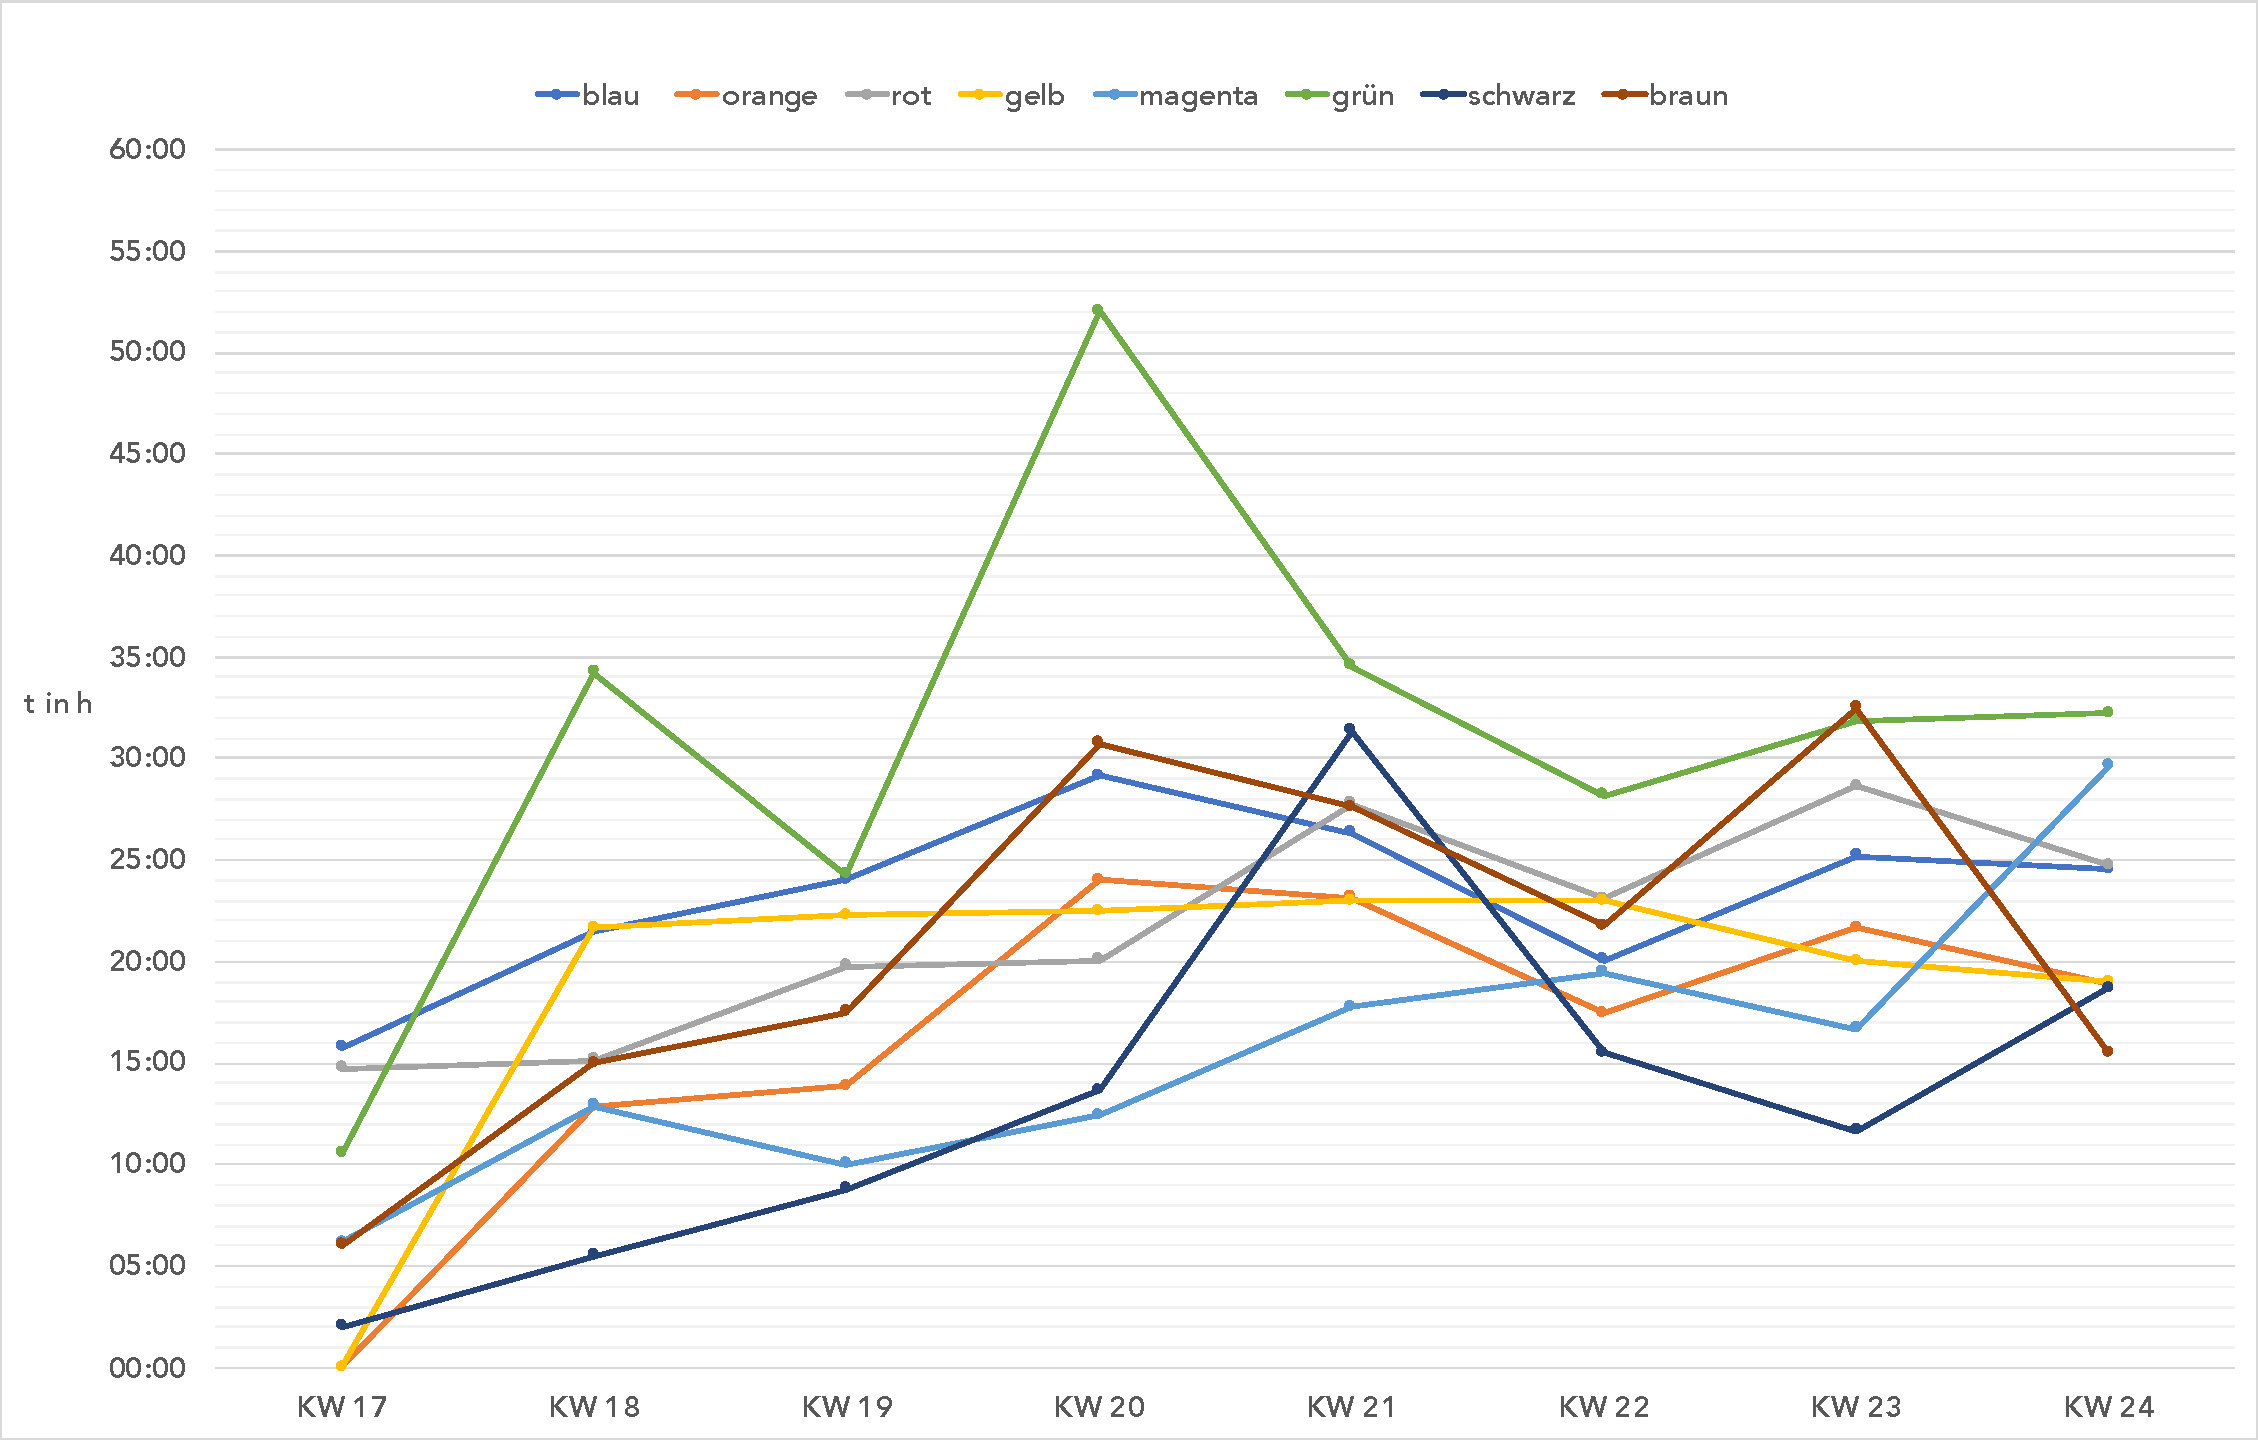
\includegraphics[width = 0.9\linewidth, trim=10pt 10pt 10pt 10pt, clip]{img/kimai10.pdf}
    \caption{Planungs- und Entwurfsphase und Implementierungsphase (KW 17-24): Zeitaufwand der einzelnen Teammitglieder}
    \label{kimai10}
\end{figure}

Die Abbildung \ref{kimai10} zeigt den Zeitaufwand der einzelnen Teammitglieder in den Kalenderwochen 17 bis 24. In den Kalenderwochen 17 bis 21 (Planungs- und Entwurfsphase) ist grundsätzlich ein Anstieg bei den meisten Teammitgliedern zu sehen. In den folgenden Wochen (Implementierungsphase) ist dieser nicht mehr so stark zu erkennen. Auch nimmt in den Kalenderwochen 22 bis 24 der Abstand zwischen den einzelnen Punkten in der Abb. \ref{kimai10} ab. Das heißt, dass der Zeitaufwand der einzelnen Teammitglieder sich nicht mehr so stark unterscheidet wie das zum Beispiel in KW 20 der Fall ist. So liegt etwa die Spannweite in KW 20 bei über 39 Stunden, während in KW 22 diese bei unter 13 Stunden liegt.
\begin{align*}
    R_{KW20} = 52h\: 1min - 12h\: 25min = 39h\: 36min
\end{align*}
\begin{align*}
    R_{KW22} = 28h\: 10min - 15h\: 19min = 12h\: 51min
\end{align*}
Der maximale Wert an Wochenstunden pro Person bleibt in KW 20 mit über 52 Stunden (vgl. Abb. \ref{kimai12}).

\begin{figure} [H]
    \centering
    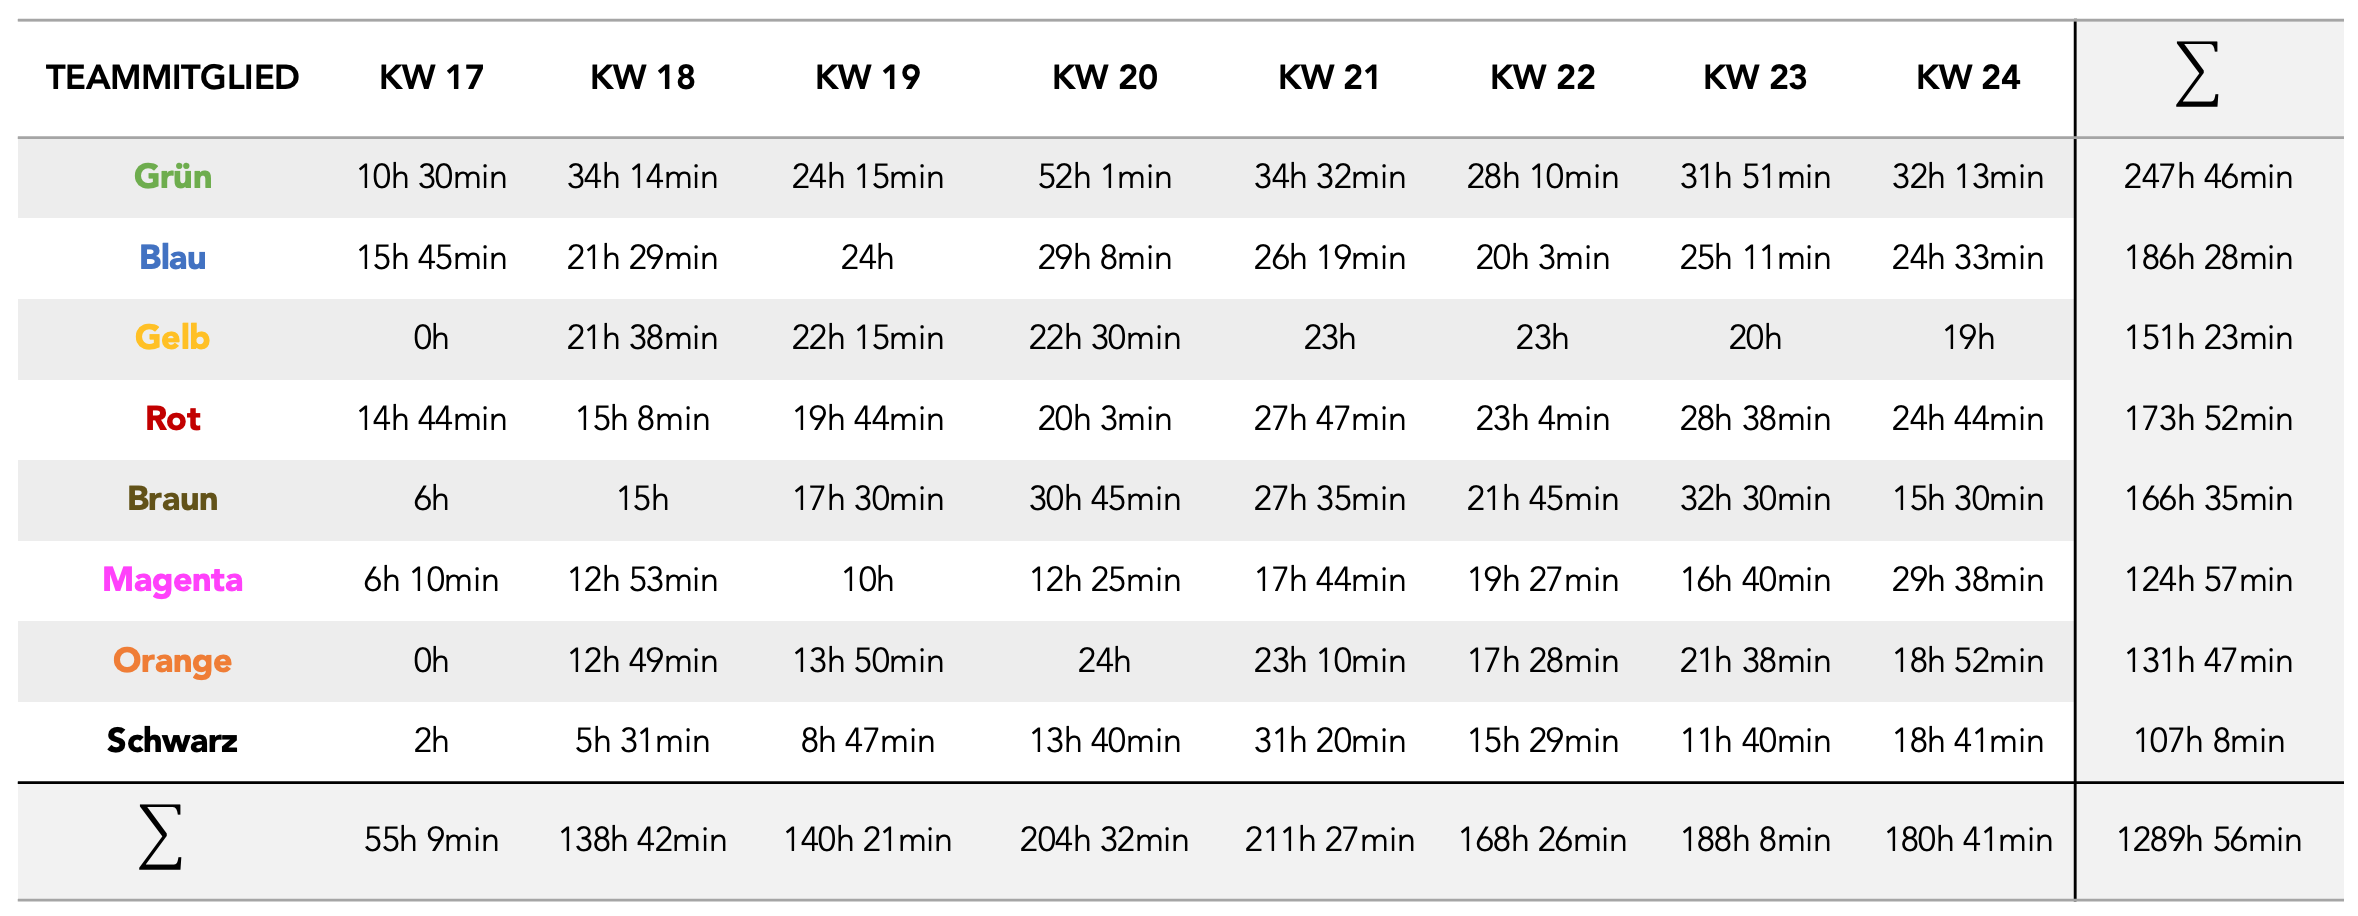
\includegraphics[width = 0.9\linewidth]{img/kimai12.png}
    \caption{Planungs- und Entwurfsphase und Implementierungsphase (KW 17-24): Tabelle mit den erfassten Zeiten}
    \label{kimai12}
\end{figure}

\subsection{Vergleich aller drei Phasen}

\begin{figure} [h]
    \centering
    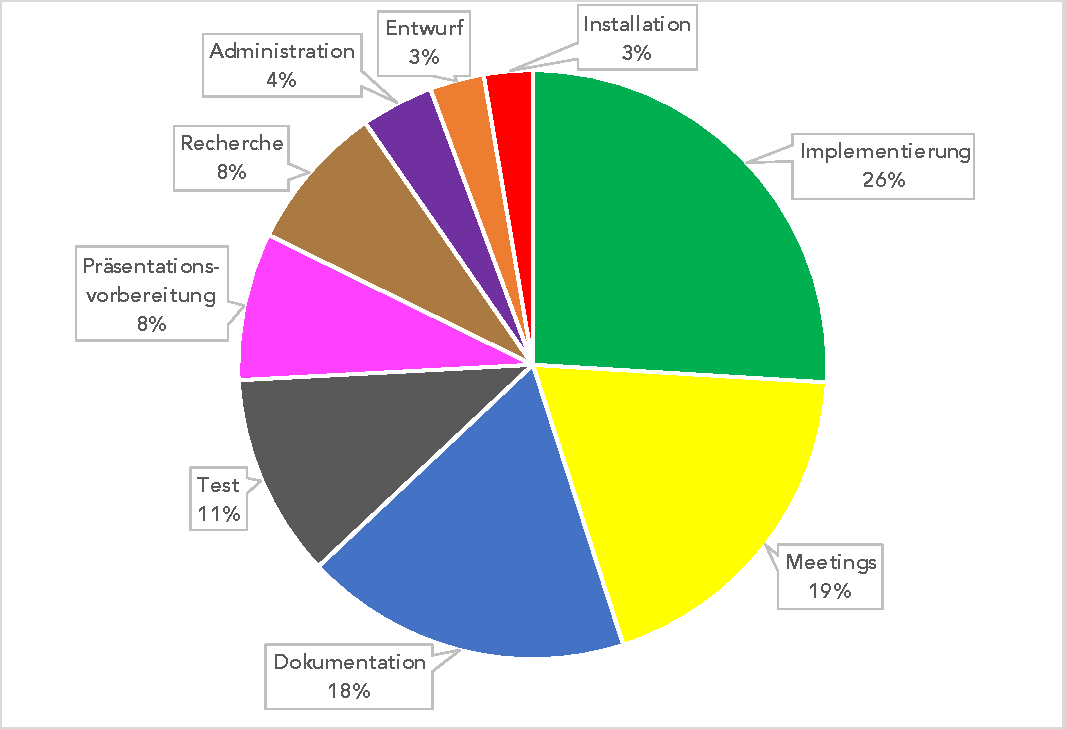
\includegraphics[width = \linewidth, trim=5pt 5pt 5pt 2pt, clip]{img/allePhasenKreis.pdf}
    \caption{Vergleich aller Phasen (KW 17-28): Anteile der Aufgabenkategorien an der insgesamt aufgebrachten Zeit}
    \label{kimai18}
\end{figure}

Das Kreisdiagramm in Abbildung \ref{kimai18} sind die Anteile aller Kategorien an der Gesamtzeit über den gesamten Zeitraum des Projekts hinweg zu sehen, wieder mit Ausnahme der letzten drei Tage.

Im Softwareprojekt wurde am meisten an der \textbf{Implementierung} gearbeitet. Rund ein Viertel der insgesamt aufgewendeten Zeit (26\%) wurde im Zeiterfassungssystem Kimai in dieser Kategorie gebucht. Während in der ersten Phase weniger als 10\% der Zeit implementiert wurde, wurde wie vom Fachgebiet System- und Software-Engineering vorgesehen in der Implementierungsphase am meisten Zeit dafür verwendet. In der Validierungsphase sank dieser Wert wieder, allerdings nicht so sehr, wie ursprünglich erhofft. Aufgrund der Komplexität des Projekts stellt es allerdings kein Problem dar, dass die Implementierung nicht in der jeweiligen Phase abgeschlossen wurde. Mit diesem Wert können die Teammitglieder also insgesamt zufrieden sein.

Etwa ein Fünftel der gesamten Zeit wurde für die \textbf{Meetings} gebucht, 19\% um genau zu sein. Nach den anfänglichen Problemen konnte dieser Anteil in der Implementierungsphase gesenkt werden. Das Team hat es geschafft, diesen Trend auch in der letzten Phase des Projekts fortführen zu können. Entscheidend dafür ist vermutlich, dass die richtigen Maßnahmen getroffen und auch umgesetzt werden. Detailliertere Infos zu diesem Thema können auch dem vorherigen, gegen Ende der Implementierungsphase erstellten Kapitel entnommen werden.

Knapp danach kommt bei dieser absteigenden Sortierung die \textbf{Dokumentation} mit 18\%. Es kann noch hinzugefügt werden, dass immer gegen Ende einer Phase mehr Zeit in dieser Kategorie gebucht wurde als am Anfang, was wahrscheinlich aus der vermehrten Arbeit am Reviewdokument resultiert.

11\% der insgesamt aufgebrachten Zeit wurde für das \textbf{Testen} genutzt. Vor allem gegen Ende des Projekts hätte womöglich noch etwas mehr getestet werden können. Es muss jedoch auch an dieser Stelle angemerkt werden, dass einige für das Testen aufgewendete Zeit in der Kategorie Implementierung gebucht worden ist.

Die \textbf{Präsentationsvorbereitung} hat insgesamt 8\% der Zeit in Anspruch genommen. Wie bereits in den vorhergehenden Kapiteln beschrieben wurde, war der Anteil dieser Kategorie aufgrund der zum Thema hinführenden Kurzvorträge zu Beginn des Projekts am höchsten. Insgesamt kann hiermit festgehalten werden, dass auch die Anteile dieser Kategorie durchaus zufriedenstellend sind.

Auch der Anteil der \textbf{Recherche} ist mit 8\% vollkommen in Ordnung.

Der geringe \textbf{Administrationsaufwand} von 4\% zeugt von einer hohen Effizienz bei administrativen Aufgaben über das gesamte Projekt hinweg.

Der ähnlich niedrige Wert für den \textbf{Entwurf} (3\%) wurde in anderen Kapiteln schon ausführlich genug behandelt. Es ist definitiv angemessen, dass in der letzten Projektphase nicht mehr viel Zeit in dieser Kategorie gebucht wurde.

Nach allen Projektphasen beläuft sich der Wert für die \textbf{Installation} ebenfalls auf 3\%. Dieser Anteil ist durchaus positiv zu bewerten.

\begin{figure} [h]
    \centering
    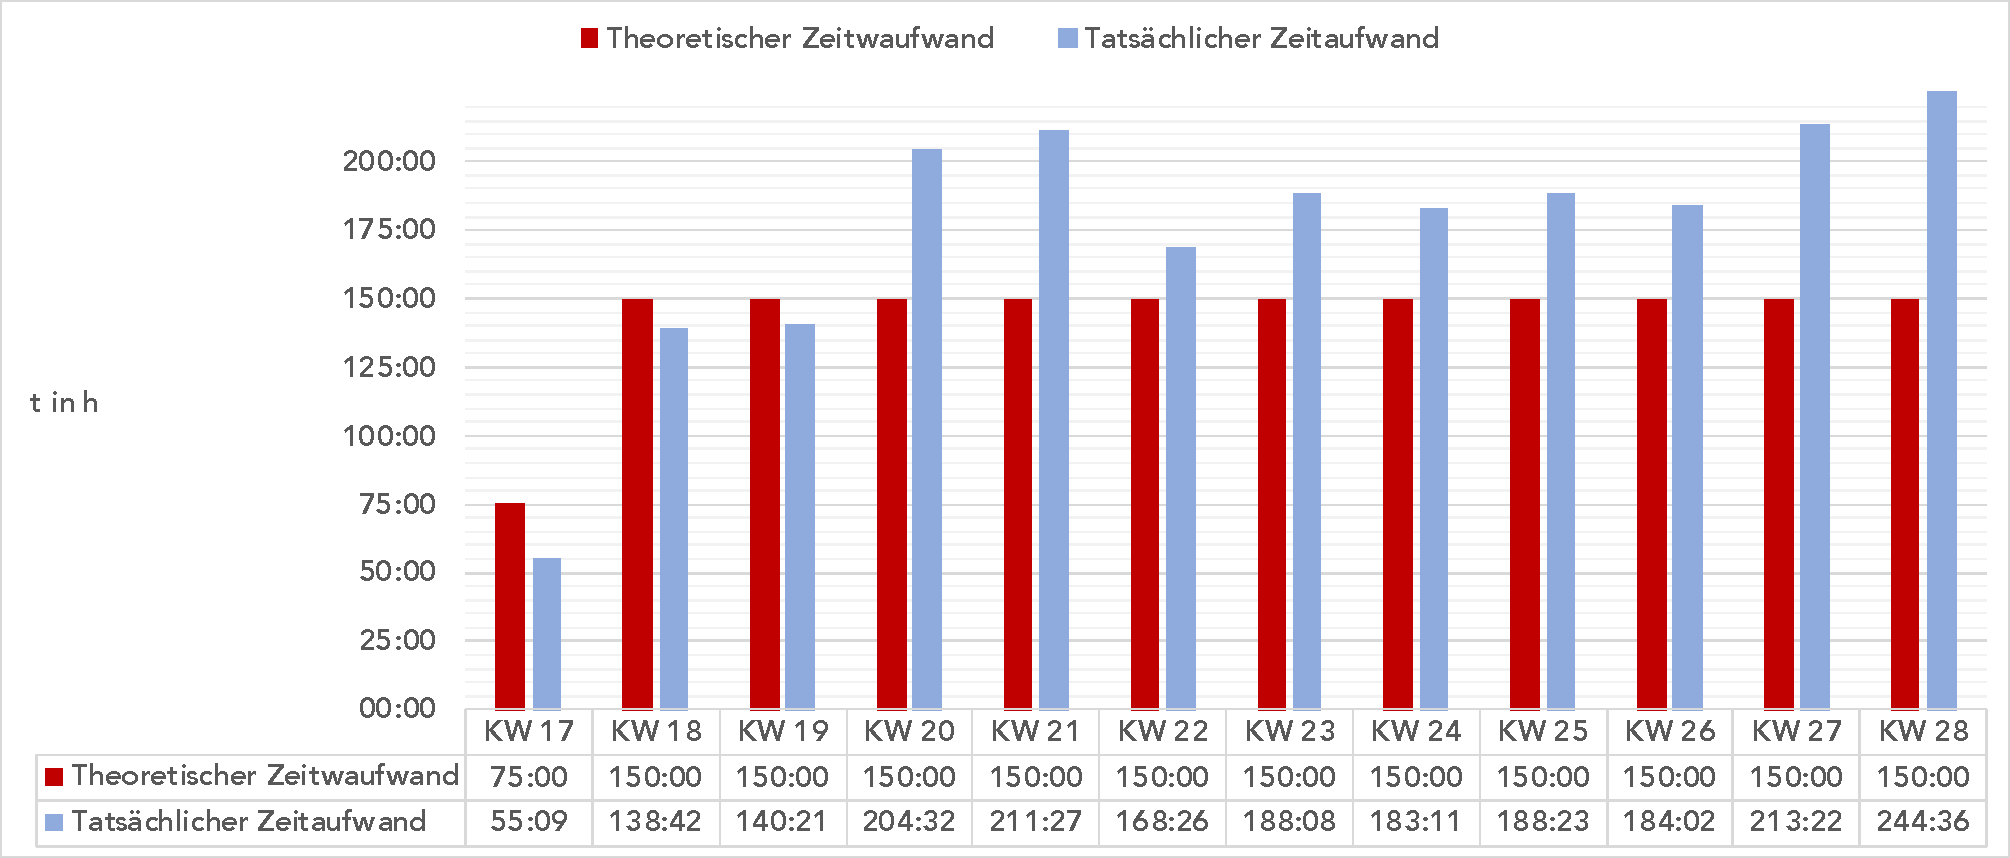
\includegraphics[width = \linewidth, trim=5pt 5pt 5pt 5pt, clip]{img/allephasen.pdf}
    \caption{Vergleich aller Phasen (KW 17-28): Vergleich des theoretischen Aufwands mit dem tatsächlichen Aufwand}
    \label{kimai15}
\end{figure}

Zu den in den vorherigen Kapiteln zu findenden Überlegungen zum Vergleich des theoretischen Aufwands mit dem tatsächlichen lässt sich nicht mehr viel hinzufügen. Eine Übersicht für das gesamte Projekt kann sowohl in Abb. \ref{kimai15} als auch in \ref{kimai17} gefunden werden. Nach ziemlich geringem tatsächlichen Aufwand zu Beginn überstieg das tatsächliche Pensum das Mindeste in jeder Woche. Womöglich ist einigen Studierenden zu Beginn des Projekts nicht wirklich bewusst gewesen, wie viel Arbeit dieses wirklich erfordert. Das hat sich im Laufe des Projekts verbessert. Zu Beginn wurde allerdings auch noch nicht die gesamte aufgebrachte Zeit im Kimai-System gebucht.

\begin{figure} [h]
    \centering
    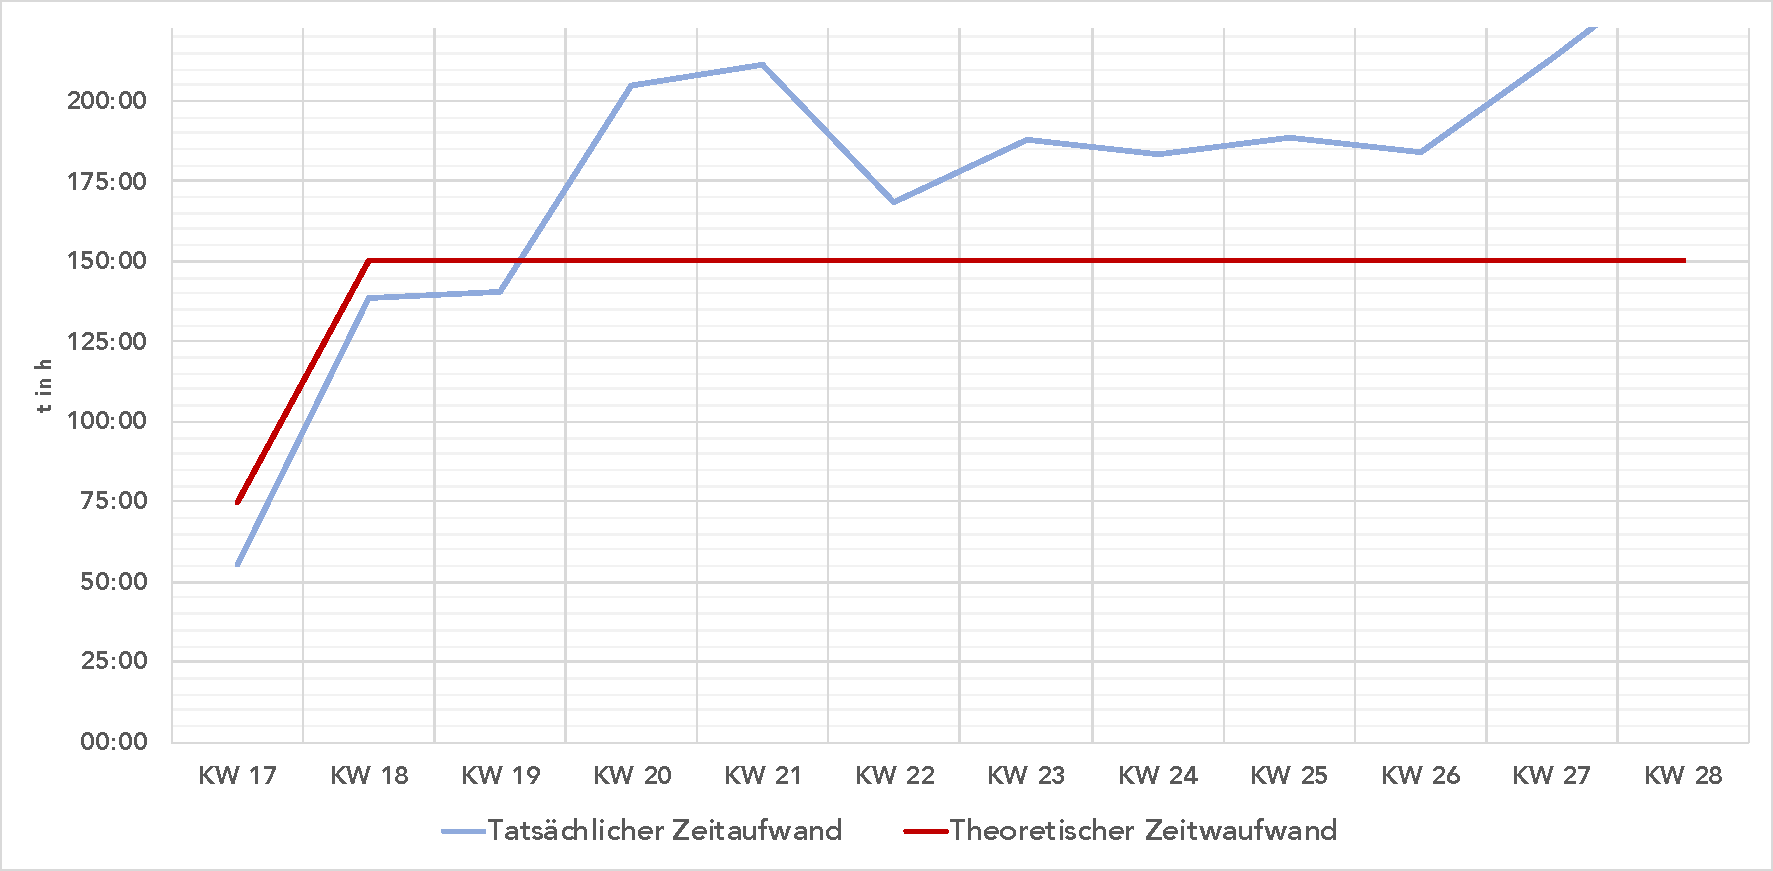
\includegraphics[width = \linewidth, trim=5pt 5pt 5pt 5pt, clip]{img/allephasen2.pdf}
    \caption{Vergleich aller Phasen (KW 17-28): Vergleich des theoretischen Aufwands mit dem tatsächlichen Aufwand als Liniendiagramm}
    \label{kimai17}
\end{figure}

In der Abbildung \ref{kimai16} wird die Verteilung der Gesamtzeit auf die einzelnen Teammitglieder dargestellt. Das Maximum über das gesamte Projekt hinweg wurde nach wie vor in der Planungs- und Entwurfsphase aufgestellt. Es lässt sich festhalten, dass sich das wöchentlichen Arbeitspensum mit Verlauf des Projekts etwas stabilisiert hat und gegen Ende weniger schwankt. Auch fällt auf, dass einzelne Teammitglieder dauerhaft mehr am Projekt gearbeitet haben als andere. Insgesamt ist die aufgebrachte Zeiten der Studierenden (siehe Abb. \ref{kimai22}) sehr zufriedenstellend. Weitere Ausarbeitungen zum Aufwand können im folgenden Kapitel gefunden werden.

\begin{figure} [h]
    \centering
    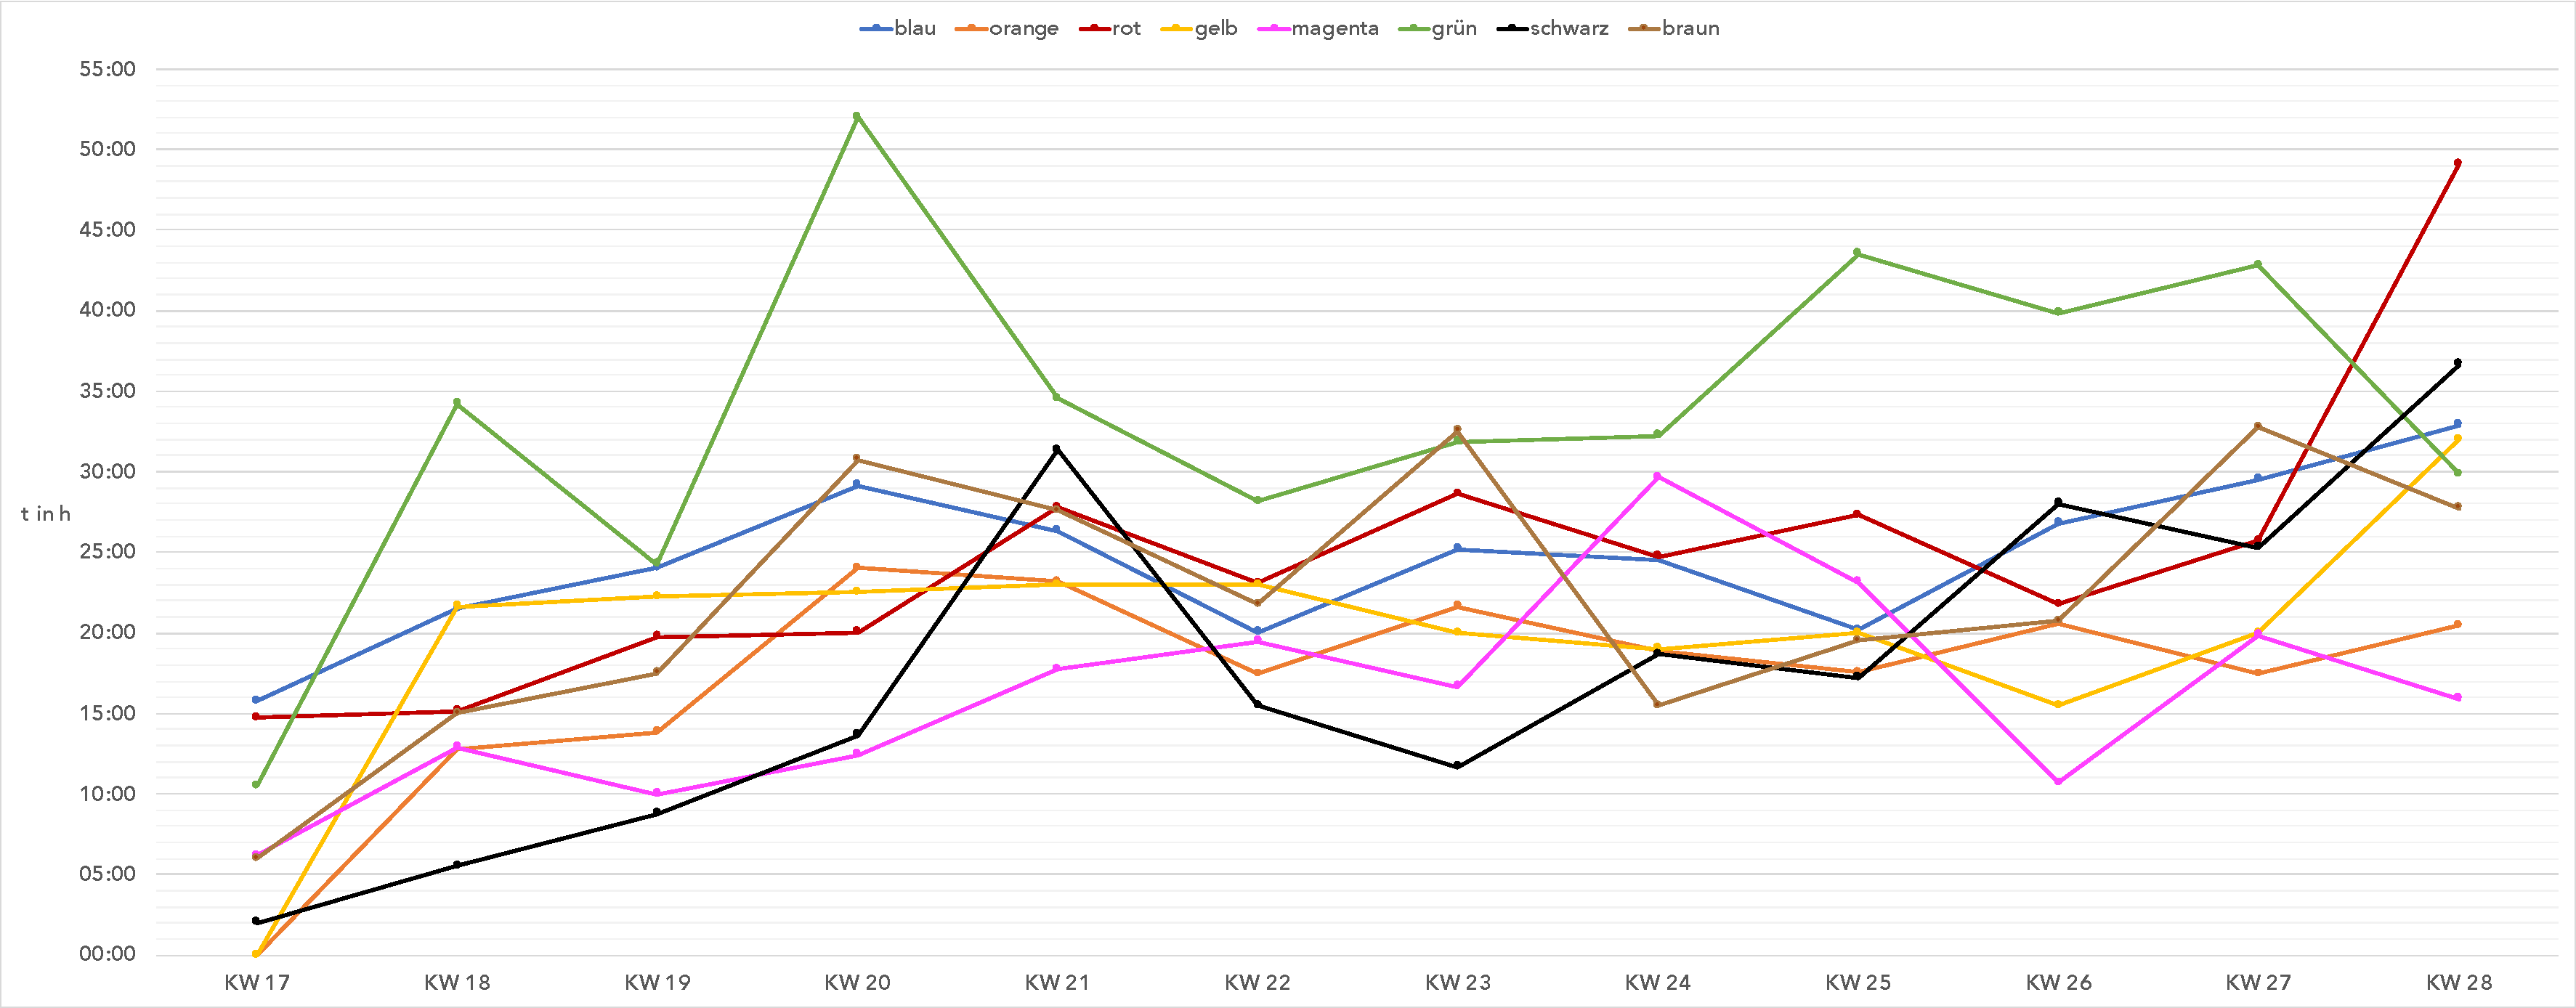
\includegraphics[width = \linewidth, trim=5pt 5pt 5pt 5pt, clip]{img/zeiten1.pdf}
    \caption{Vergleich aller Phasen (KW 17-28): Zeitaufwand der einzelnen Teammitglieder}
    \label{kimai16}
\end{figure}

\begin{figure} [h]
    \centering
    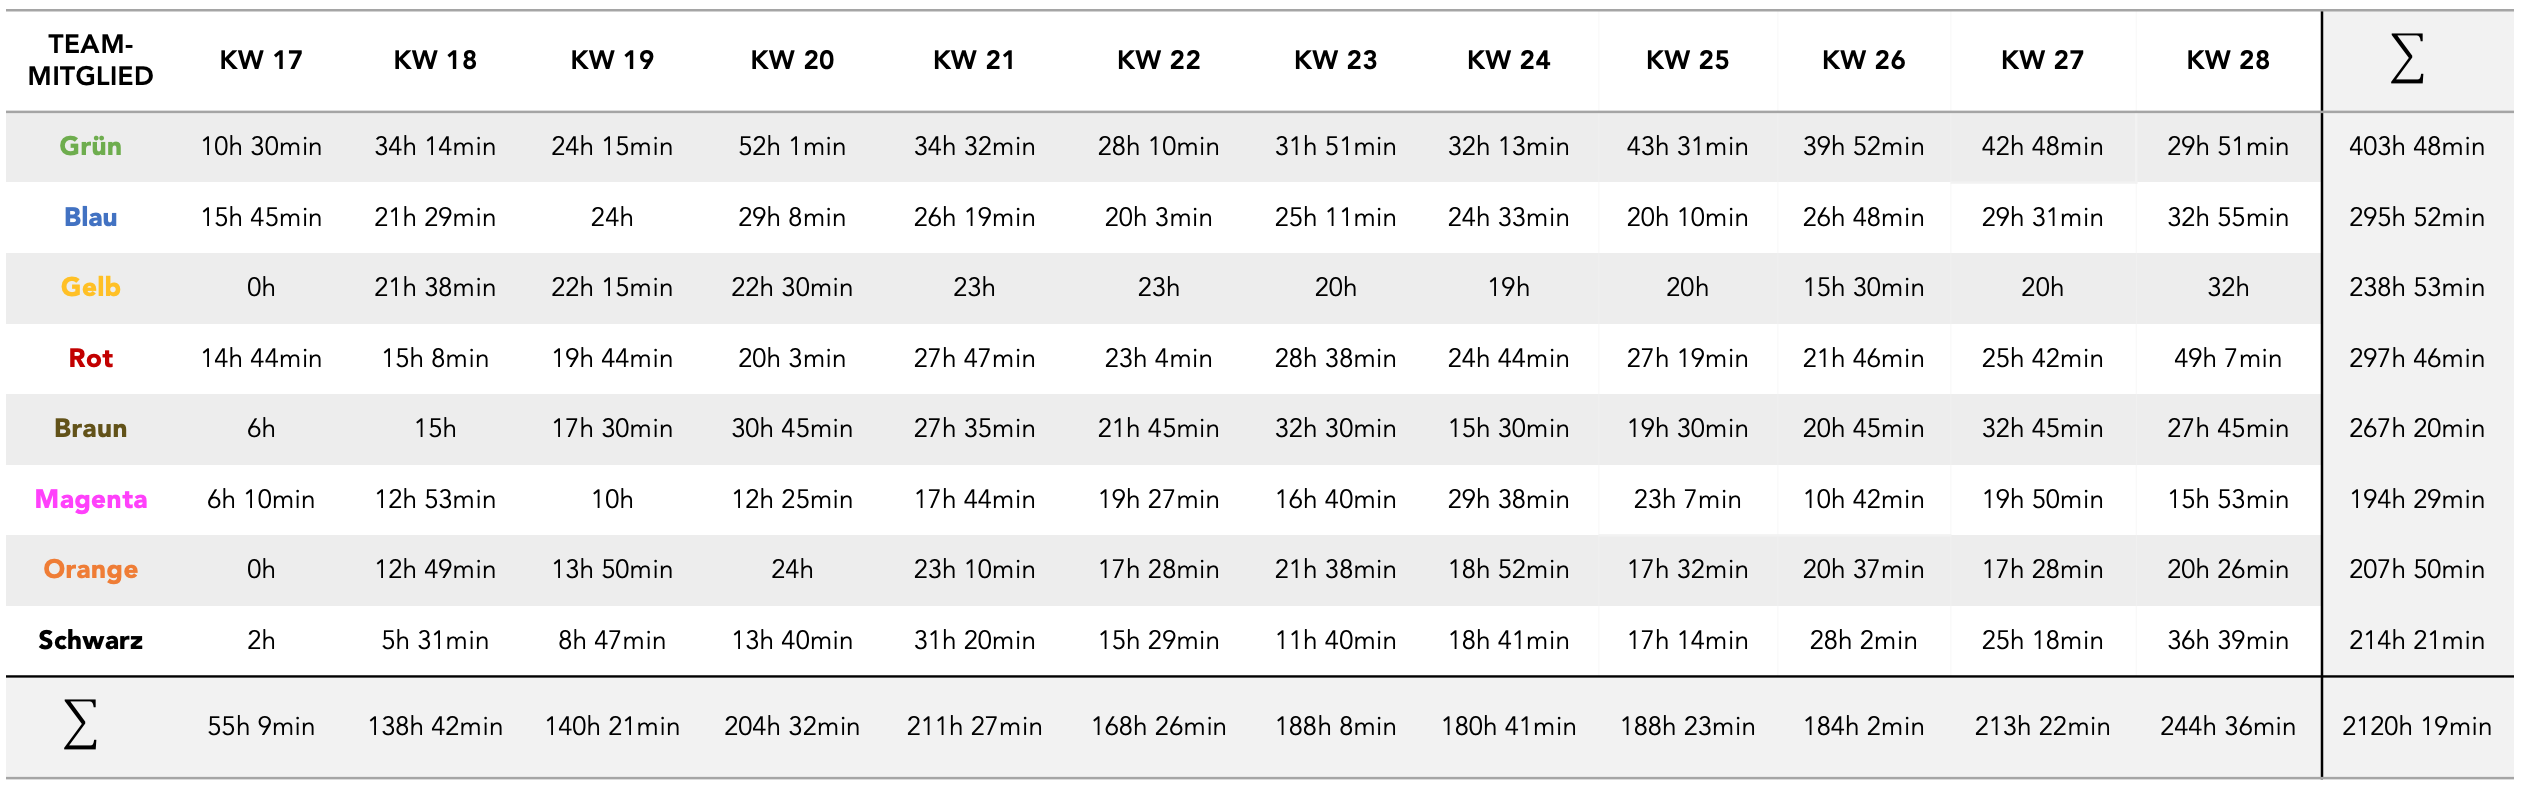
\includegraphics[angle=270, width = 0.42\linewidth]{img/tabelle2.png}
    \caption{Alle Phasen (KW 17-28): Tabelle mit den erfassten Zeiten}
    \label{kimai22}
\end{figure}

\section{Validierung der Aufwandsschätzung der Planungs- und Entwurfsphase}
Im Abschnitt \glqq \nameref{kap1}\grqq{} wird zunächst das Aufwandsschätzverfahren COCOMO II  kurz vorgestellt. Die dort erhaltenen Ergebnisse werden im Abschnitt  \glqq \nameref{kap2}\grqq{} mit dem tatsächlichen Aufwand verglichen. Dieser IST-Aufwand berechnet sich aus den von den Teammitgliedern in die Zeiterfassungs-Software Kimai eingetragenen Zeiten.

\subsection{Aufwandsschätzung nach dem COCOMO II aus der Planungs- und Entwurfsphase} \label{kap1}
Bei COCOMO II (COnstrucitve COst MOdel), welches bereits 1981 durch den Softwareingenieur Barry W. Boehm entwickelt wurde, handelt sich es um ein algorithmisches Modell zur Aufwandsschätzung von Software. In diesem Modell werden zahlreiche Einflussfaktoren wie Quantität, Qualität oder Produktivität berücksichtigt. Zudem besteht COCOMO II aus drei Teilmodellen, welche sich unter anderem in den Skalenfaktoren oder den Modellkonstanten unterscheiden. Im Folgenden wird sich auf \textit{\glqq The Early Design Model\grqq{}} (Die frühe Entwicklungsstufe) bezogen, da diese Stufe stark zum derzeitigen Projektstand passt. Auf dieser Stufe liegen schon sowohl die Anforderungen als auch ein erster Grobentwurf vor.

Das Modell baut im Wesentlichen auf folgender Formel auf:
\begin{align}
    PM = A \cdot \text{Größe}^E \cdot M
    \label{formel1}
\end{align}
Für den Koeffizienten A wird der Erfahrungswert 2,5 angenommen.
Die Größe wird in KLSLOC (kilo source lines of code) angegeben. Sie beträgt hier 3,6. Als Referenzprojekt dient POSEIDON\cite{testFab}.
In diesem Projekt wurde eine DDoS-Abwehr durch ungefähr 3600 C/C++-Codezeilen implementiert. Im Unterschied zu der hier zu entwickelnden Software wurde jedoch ein komplettes Endprodukt entwickelt und kein Prototyp, wie es in dem vorliegenden Projekt der Fall ist.
Um den steigenden Aufwand bei wachsender Projektgröße zu berücksichtigen, wird der Exponent E, dessen Wert zwischen 1,01 und 1,26 liegt, verwendet. Durch die Bewertung unterschiedlicher Skalierungsfaktoren wird E berechnet.

\begin{longtable}[h] {l c p{8.0cm}}
    \toprule
    \textbf{Faktor}              & \textbf{Punkte} & \textbf{Bemerkungen}                                                                                                                                                                                                                                  \\ \midrule \endhead
    Neuartigkeit                 & 2               & Bei einzelnen Teammitgliedern liegt noch geringe Erfahrung mit dieser Art von Projekten vor. Dies ist oftmals begründet durch das junge Alter. Jedoch gibt es online schon Lösungen zu ähnlichen Problemen vor, an denen sich orientierenwerden kann. \\
    Entwicklungsflexibilität     & 2               & Zwar liegen einige Vorgaben zum Ablauf des SW-Projektes vor (z.B. die Einteilung in drei Hauptphasen), jedoch erlaubt das Vorgehensmodell Unified Process noch eine gewisse Flexibilität im Entwicklungsprozess.                                      \\
    Architektur/ Risikoauflösung & 3               & Die Risiken wurden rechtzeitig identifiziert und Maßnahmen überlegt. Jedoch könnten aufgrund der geringen Erfahrung noch Risiken unentdeckt geblieben sein.                                                                                           \\
    Teamzusammenhalt             & 1               & Die Vertrautheit und Zusammenarbeit im Team ist optimal.                                                                                                                                                                                              \\
    Ausgereiftheit des Prozesses & 5               & Der Prozess ist noch wenig ausgereift.                                                                                                                                                                                                                \\ \bottomrule
\end{longtable}

E lässt sich nun berechnen, indem auf den fixen Wert 1,01  ein Hundertstel von der Summe der Punkte addiert wird.
\begin{align*}
    E = 1,01 + \frac{2+2+3+1+5}{100}= 1,01 + 0,13 = 1,14
\end{align*}
M ergibt sich durch die Multiplikation folgender Projekt- und Prozessfaktoren:
\begin{itemize}
    \setlength\itemsep{-1mm}
    \item RCPX: Product Reliability and Complexity
    \item RUSE: Developed for Resuability
    \item PDIF: Platform Difficulty
    \item PERS: Personnel Capability
    \item PREX: Personnel Experience
    \item FCIL: Facilities
    \item SCED: Required Developement Schedule
\end{itemize}
Mithilfe der unteren Skala werden die einzelnen Projekt- und Prozessfaktoren bewertet. In der Farbe Rot sind diejenigen Faktoren gekennzeichnet, die auf das vorliegende Projekt am besten zutreffen.

\begin{center}
    \begin{tabular} [h] {|l|c|c|c|c|c|c|c|}
        \hline & \textbf{- - -} & \textbf{- -}          & \textbf{-}            & \textbf{\textasciitilde} & \textbf{+}            & \textbf{++} & \textbf{+++} \\ \hline
        RCPX   & 0,49           & 0,60                  & 0,83                  & 1                        & \textcolor{red}{1,33} & 1,91        & 2,72         \\ \hline
        RUSE   &                &                       & \textcolor{red}{0,95} & 1                        & 1,07                  & 1,15        & 1,24         \\\hline
        PDIF   &                &                       & \textcolor{red}{0,87} & 1                        & {1,29}                & 1,81        & 2,61         \\ \hline
        PERS   & 2,12           & 1,62                  & {1,26}                & \textcolor{red}{1}       & 0,83                  & 0,63        & 0,50         \\ \hline
        PREX   & 1,59           & \textcolor{red}{1,33} & 1,22                  & 1                        & 0,87                  & 0,74        & 0,63         \\ \hline
        FCIL   & 1,43           & 1,30                  & 1,10                  & \textcolor{red}{1}       & 0,87                  & 0,73        & 0,62         \\ \hline
        SCED   &                & 1,43                  & {1,14}                & \textcolor{red}{1}       & 1                     & 1           & n/a          \\ \hline
    \end{tabular}
\end{center}
Nun lässt sich der Multiplikator M berechnen:
\begin{align*}
    M = PERS \cdot RCPX \cdot RUSE \cdot PDIF \cdot PREX \cdot FCIL \cdot SCED \\= 1,33 \cdot 0,95 \cdot 0,87 \cdot1 \cdot 1,33 \cdot 1 \cdot 1 \approx 1,22
\end{align*}
Jetzt sind alle Werte gegeben, um mithilfe der Formel \ref{formel1} den Aufwand in Personenmonate zu schätzen.
\begin{align*}
    PM = A \cdot \text{Größe}^E \cdot M = 2,5 \cdot 3,6 \textsuperscript{1,14} \cdot1,22 \approx 13,17
\end{align*}
Nun kann der Aufwand in Personenmonat in Personenstunden umgerechnet werden die Folgende:
\begin{align*}
    PS= 13,17 \cdot 160h = 2107h
\end{align*}
Das Team besteht aus zwei Wirtschaftsinformatikern, die jede Woche 15 Stunden für das Softwareprojekt aufwenden sollen, sowie sechs Informatiker und Ingenieurinformatiker, deren Wochenstundenanzahl bei 20 Stunden liegt. Das Softwareprojekt soll innerhalb von 12 Wochen beendet werden.

Somit ist die zur Verfügung stehende Zeit:
\begin{align*}
    (2\cdot15 h+6\cdot20 h)\cdot12=1800h
\end{align*}
\textbf{Interpretation der Ergebnisse:}

Der Wert von 2107 Stunden liegt ca. 300 Stunden über dem angestrebten Wert von 1800 Stunden. Es kann unterschiedliche Gründe für diese Abweichung geben.

Ein Grund dafür könnte sein, dass im zu entwickelnden System kein schlüsselfertiges Produkt entwickeln wird, sondern vielmehr ein Prototyp. Somit könnte der Schätzwert von 3600 Codezeilen zu hoch gegriffen sein.

Durch die Komplexität des Projektes kann es zudem vorkommen, dass die 15 beziehungsweise 20 Wochenstunden nicht immer ausreichend sind und somit mehr Arbeitszeit aufgewendet werden muss.
Zudem muss keine Zeit zur Berücksichtigung von Support vorgesehen werden, da es nach den 12 Wochen als abgeschlossen angesehen werden kann.

Bereits kleine Änderungen an den Projekt- und Prozessfaktoren haben große Auswirkungen. Falls bereits einer dieser oben aufgeführten Faktoren ungenau geschätzt wurde, kann das Ergebnis verfälscht sein.
Abschließend kann noch angemerkt werden, dass es sich um eine Schätzung handelt. Schätzungen sind (fast) immer mit Ungenauigkeiten verbunden.

\subsection{Vergleich der Ergebnisse aus der Aufwandsschätzung mit dem tatsächlichen Aufwand} \label{kap2}

Um die Ergebnisse der Aufwandsschätzung mit dem tatsächlichen (zeitlichen) Aufwand zu vergleichen, werden zunächst alle eingetragenen Werte aus der Zeiterfassungssoftware addiert. Da diese Auswertung bereits in KW 28 stattfand, stehen hier nur die genauen Werte von KW 17 bis KW 27 zur Verfügung. Der Zeitaufwand für die Wochen KW 28 und KW 29 wird aus den Vergangenheitswerten prognostiziert.

\begin{longtable} [h] {l r} \toprule
    \textbf{Kalenderwoche} & \textbf{Zeitaufwand des Teams in [h:min]} \\ \midrule \endhead
    KW 17                  & 55:09                                     \\
    KW 18                  & 138:42                                    \\
    KW 19                  & 140:21                                    \\
    KW 20                  & 204:32                                    \\
    KW 21                  & 211:27                                    \\
    KW 22                  & 168:26                                    \\
    KW 23                  & 188:08                                    \\
    KW 24                  & 183:11                                    \\
    KW 25                  & 188:23                                    \\
    KW 26                  & 184:02                                    \\
    KW 27                  & 213:22                                    \\  \midrule
    $\sum$                 & 1875:43                                   \\ \bottomrule
\end{longtable}

Um den Aufwand für KW 28 und KW 29 zu schätzen, wird der Mittelwert des Zeitaufwandes der Kalenderwochen 18 bis 27 ermittelt. KW 17 fließt nicht in die Rechnung mit einem. Der Grund liegt zum einen darin, dass in dieser Woche das Projekt erst am Donnerstag gestartet war und somit die Woche verkürzt war. Zum anderen stand in dieser Woche das Tool Kimai noch nicht zur Verfügung, wodurch die Zeiten von den Projektmitgliedern in der darauffolgenden Woche nachgetragen werden mussten. Das hatten jedoch nicht alle gemacht.

Die Variable x steht im Folgenden für die Kalenderwoche, die Variable y für die Zeit. Die Variable y wurde auf zwei Nachkommastellen genau berechnet.
\begin{longtable} [h] {l r} \toprule
    \textbf{x} & \textbf{y} \\ \midrule \endhead
    17         & 55,15      \\
    18         & 138,70     \\
    19         & 140,35     \\
    20         & 204,53     \\
    21         & 211,45     \\
    22         & 168,43     \\
    23         & 188,13     \\
    24         & 183,18     \\
    25         & 188,38     \\
    26         & 184,03     \\
    27         & 213,22     \\\midrule
    $\sum$     & 1875,72    \\
    -17        & 55,15      \\ \midrule
    $\sum$     & 1820,57    \\ \bottomrule
\end{longtable}

Der (gerundete) Mittelwert berechnet sich wie folgt:
\begin{align*}
    \bar{y} = y \textsubscript{28}=  \frac{1}{n}\sum_{i=1}^{n}y_i
     & = \frac{1}{10} \cdot (138,70+140,35+204,53+211,45+168,43+188,13 +183,18 +188,38 \\+184,03+213,22)
     & = \frac{1820,57}{10} \approx 182\end{align*}
Somit wird ein Wert von 182 h für die Kalenderwoche 28 prognostiziert.

\begin{align*}
    y \textsubscript{29} = \frac{3}{7} \cdot \bar{y} = \frac{3}{7}  \cdot 182 = 78
\end{align*}
Für KW 29 ergibt sich ein geschätzter Wert von 78h.

\begin{figure} [h]
    \centering
    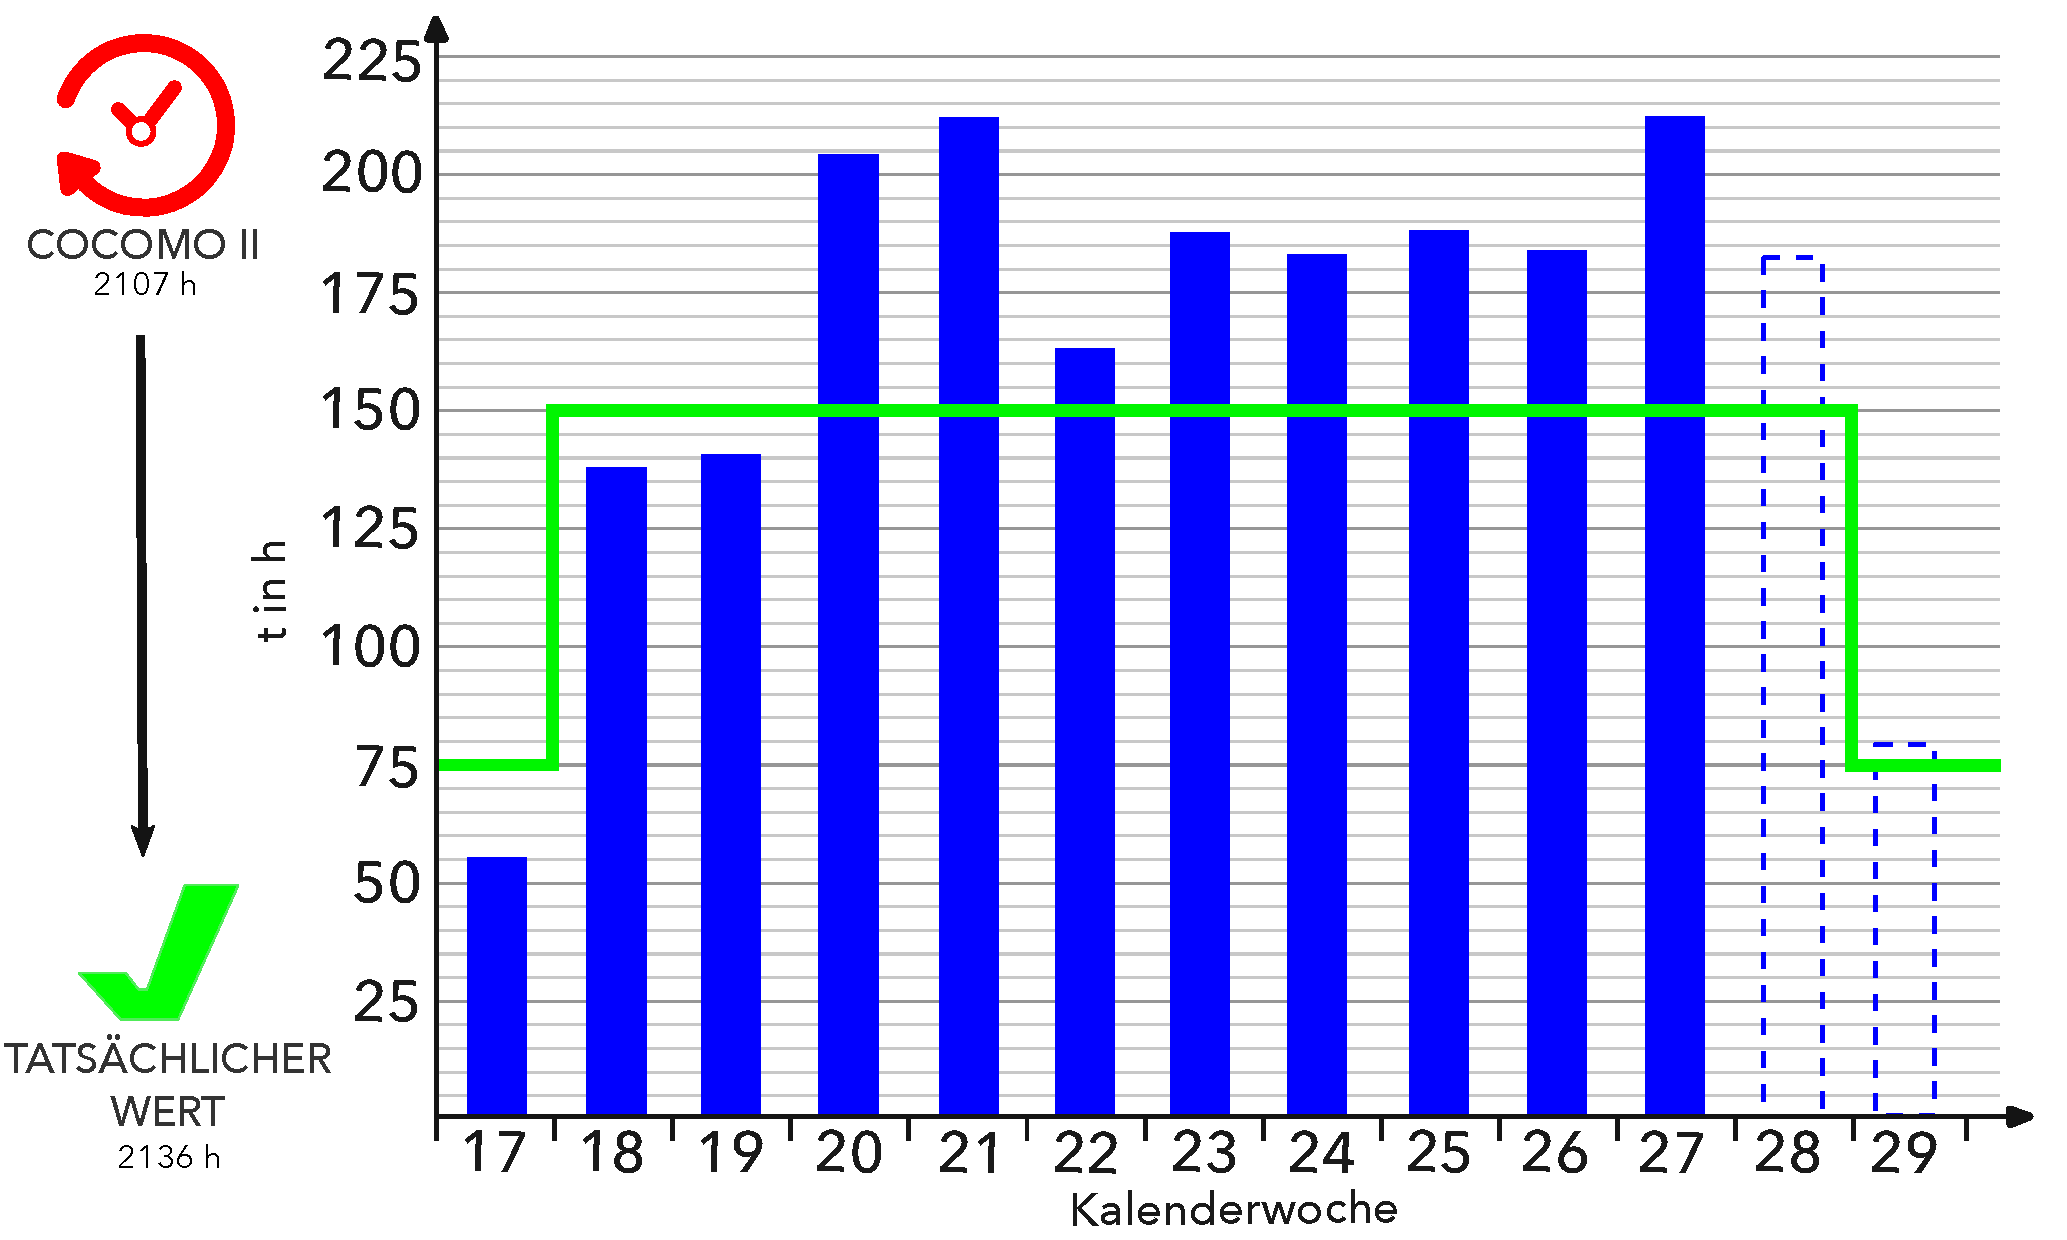
\includegraphics[width = 0.9\linewidth]{img/AufwandsschaetzungNeu.pdf}
    \caption{Tatsächlich aufgebrachte Zeit von KW 17 bis KW 27 und geschätzte Werte für KW 28 und KW 29}
    \label{aufw}
\end{figure}
Diese beiden geschätzten Werte werden nun auf die 1875h 43min aufaddiert. Das Ergebnis ist 2135h 43 min. Die Werte aller Kalenderwochen sind in Abb. \ref{aufw} visualisiert.

Wenn ein Vergleich zwischen den 2135h 43 min und dem Ergebnis der Aufwandsschätzung aus COCOMO II (2107h) gezogen werden soll, zeigt sich nur eine minimale Differenz zwischen den beiden Ergebnissen.

\section{Vergleich: Vorgehensmodell}

Zuerst wird in diesem Teilkapitel auf das idealtypische und dann auf das tatsächliche Vorgehensmodell eingegangen.

\subsection{Idealtypisches Vorgehensmodell}

Gleich zu Beginn des Projekts wurde sich für den Unified Process als Vorgehensmodell entschieden.

\begin{figure} [h]
    \centering
    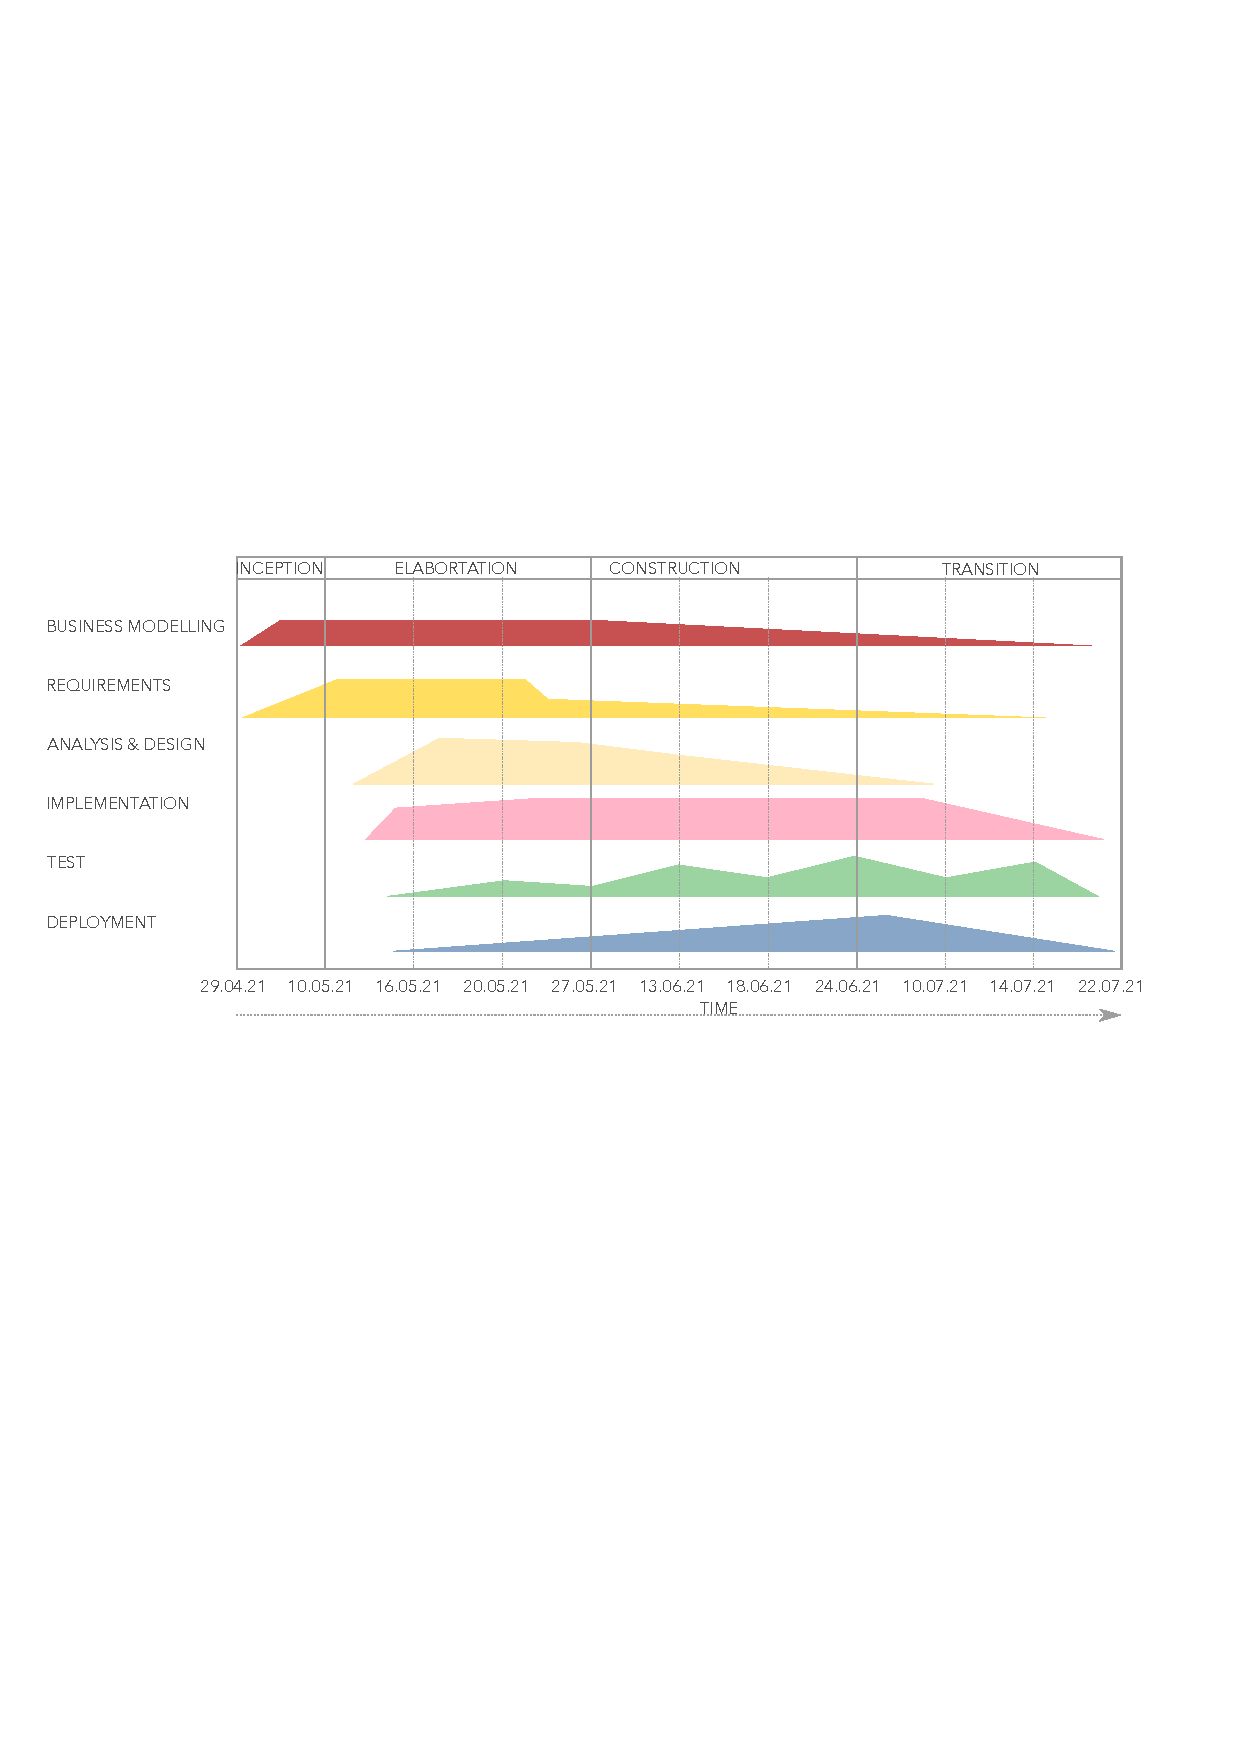
\includegraphics[width = \linewidth]{img/UnifiedProcess.pdf}
    \caption{Idealisierte Abbildung zum Vorgehensmodell Unified Process aus der Planungs-und Entwurfsphase}
    \label{up}
\end{figure}

In Abb. \ref{up} sehen ist ein idealisierter Verlauf der Kernprozesse des Projekts abgebildet. In den vier Phasen des Projekts (Inception, Elaboration, Construction, Transition) laufen verschiedene dieser Kernprozesse parallel ab.

Die Kernprozesse können wie folgt ins Deutsche übersetzt werden: Business Modelling $\widehat{=}$ Geschäftsprozessmodellierung, Requirements $\widehat{=}$ Anforderungsanalyse, Analysis and Design $\widehat{=}$ Analyse und Entwurf, Implementation $\widehat{=}$ Implementierung, Developement $\widehat{=}$ Auslieferung.

Da im Projekt die Aktivitäten, die im Kimai verbucht wurden, nicht deckungsgleich mit den obigen Kernprozessen sind, muss eine Zuordnung vorgenommen werden: Zum Entwurf zählen die Kernprozesse Analysis, Design und Business Modelling.

Die anderen Aktivitäten im Kimai (z. B. Meeting, Präsentationsvorbereitung, Dokumentation) haben keine Entsprechung in den Kernprozessen.

\subsection{Tatsächliches Vorgehensmodell}

\begin{figure} [h]
    \centering
    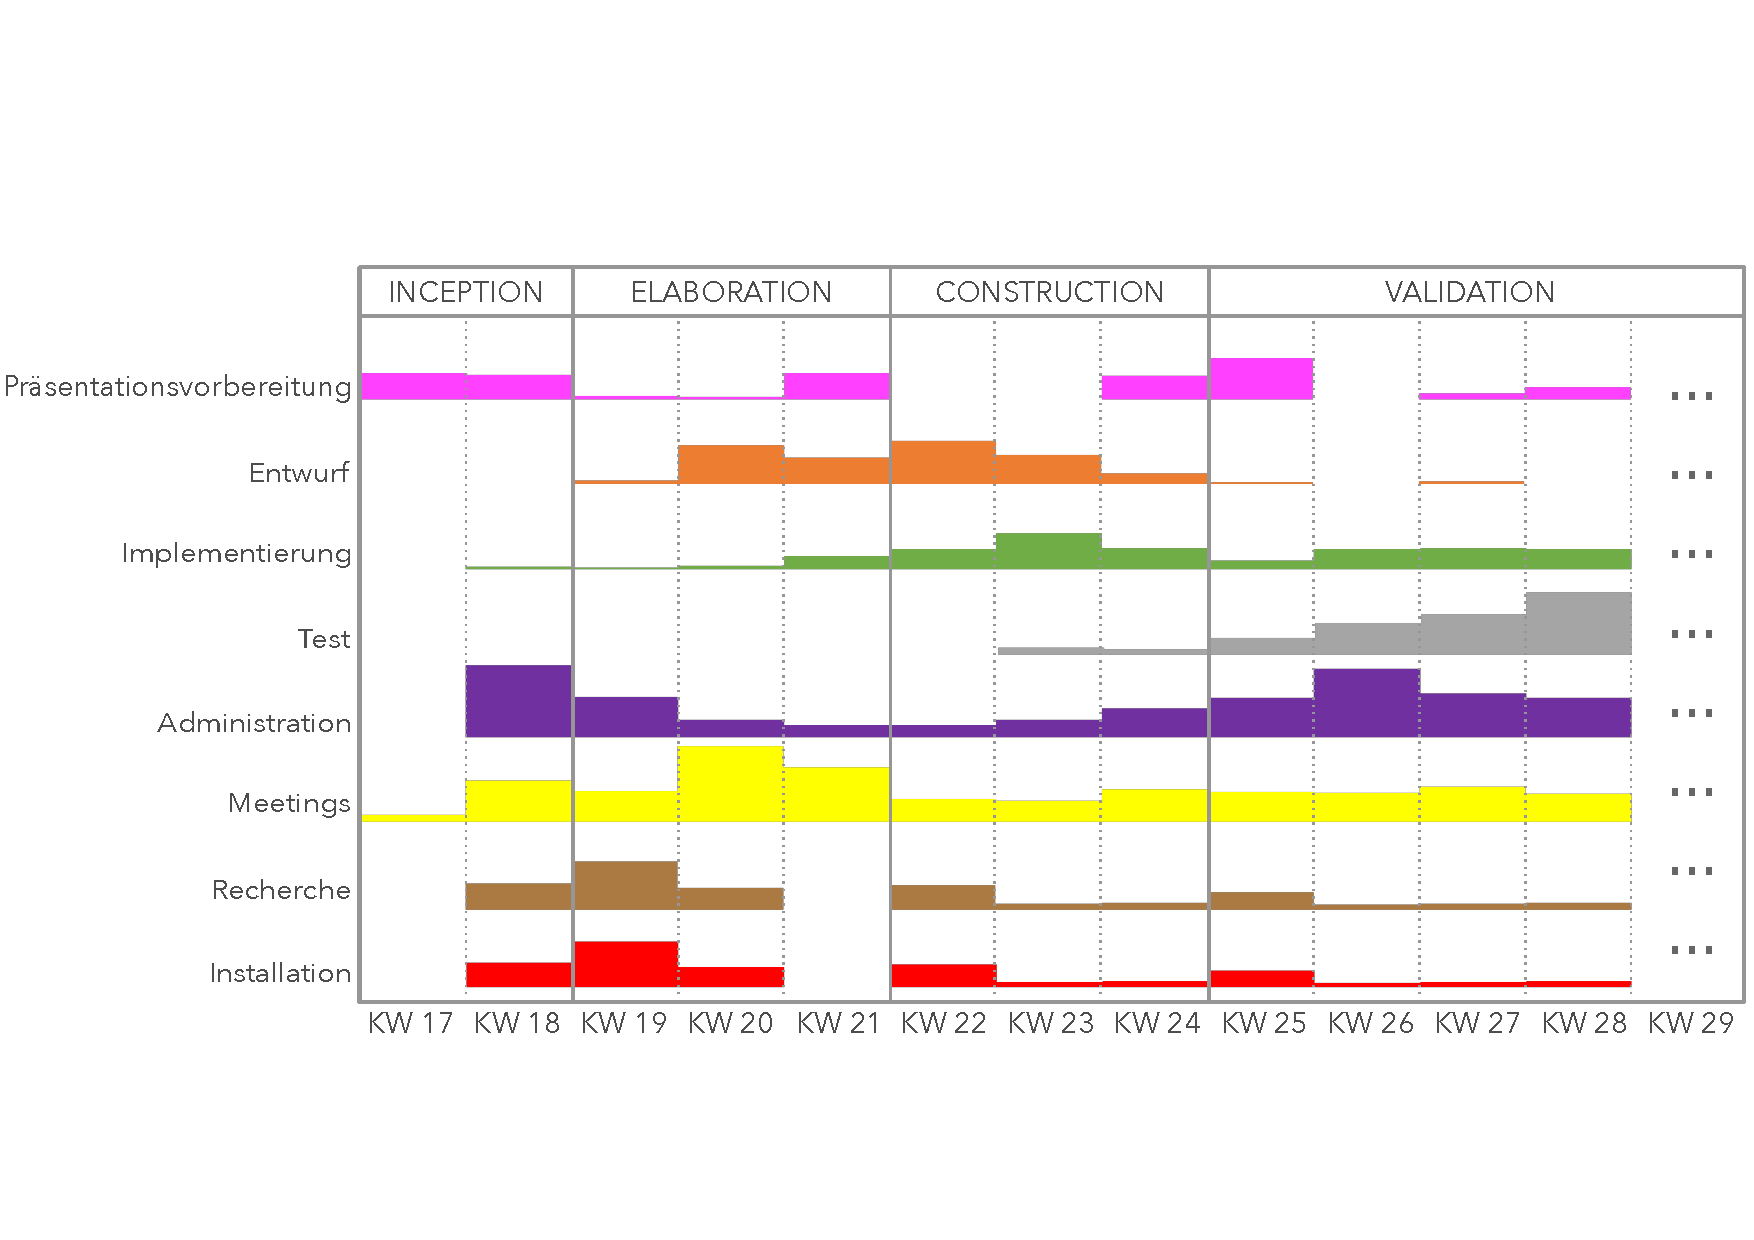
\includegraphics[width = \linewidth]{img/kimai21.pdf}
    \caption{Abbildung des tatsächlichen Vorgehens gegen Ende der Validierungsphase}
    \label{kimai21}
\end{figure}

In Abbildung \ref{kimai21} ist eine zu Abbildung \ref{up} ähnliche Abbildung zu sehen. Dabei handelt es sich allerdings nicht um das für den Unified Process idealtypische Vorgehen, sondern um das tatsächliche. Dabei zeigt die Höhe des Säule einer bestimmten Woche den Anteil der in dieser Woche für diese Kategorie aufgewendeten Zeit an der insgesamt für diese Kategorie aufgewendeten Zeit. In der Woche mit der höchsten Säule wurde demzufolge am meisten für diese Kategorie gearbeitet.

Es fällt zunächst auf, dass bereits in der Inception-Phase, also der ersten Woche des Projekts, ein großer Anteil der insgesamt für die \textbf{Präsentationsvorbereitung} gebuchten Zeit in Kimai erfasst wurde. Das liegt daran, dass hier alle Studierenden an einem von vier einleitenden Vorträgen arbeiteten. Die vier Themen werden der Vollständigkeit halber im Folgenden einmal aufgeführt:
\begin{itemize}
    %\setlength{\parskip}{-2pt}
    \item DPDK
    \item Denial-of-Service-Angriffe
    \item Effiziente Datenstrukturen
    \item git und Latex, Kimai
\end{itemize}
Außerdem sieht man, dass gegen Ende der jeweiligen Phase immer mehr an der Vorbereitung der Präsentationen gearbeitet wurde als am Anfang. Der Grund dafür ist, dass diese Vorbereitung insbesondere kurz vor den entsprechenden Reviews vorgenommen wurde. Im Diagramm stellt KW25 jedoch eine Ausnahme dar. Die in dieser Woche in der Kategorie für die Präsentationen eingetragenen Zeiten, zählen genau genommen auch zur Construction-Phase, weil das zweite Review am Donnerstag der KW25 stattgefunden hat.

Die tatsächliche Verteilung der Arbeit am \textbf{Entwurf} ähnelt sehr der idealen. Das heißt, dass in der Elaboration-Phase (v. a. Grobentwurf) mit dem Entwurf begonnen wurde und diese mit dem Abschluss der Construction-Phase (v. a. Feinentwurf) fast vollständig abgeschlossen wurde.

Auch in puncto \textbf{Implementierung} reicht das tatsächliche Vorgehen ziemlich nahe an das geplante bzw. ideale heran. Es wurde schon früh mit dem Implementieren begonnen und sowohl in Abb. \ref{up} als auch in Abb. \ref{kimai21} ist zu sehen, dass die Implementierung auch in der Validierungsphase noch nicht abgeschlossen gewesen ist.

Mit dem \textbf{Testen} hätte zwar wie in anderen Kapiteln bereits hinreichend beschrieben eher begonnen werden können. Jedoch kann positiv angemerkt werden, dass die Tests vor allem gegen Ende immer häufiger wurden, denn das ist auch beim idealisierten Unified Process so.

Der zu Beginn und gegen Ende relativ hohe \textbf{Administrationsaufwand} kann so begründet werden, dass in den frühen Phasen viele organisatorische Aspekte geklärt werden mussten.

Im ersten Monat des Projekts wurde besonders viel Zeit für \textbf{Meetings} verwendet. Wie in der Abbildung zu sehen, waren die eingeleiteten Gegenmaßnahmen jedoch die richtigen. Ab der Construction-Phase hat sich die Dauer der Meetings auf einem moderaten Niveau eingependelt.

Die Graphen für die \textbf{Recherche} und die \textbf{Installation} verlaufen beinahe identisch. Vor alle zu Beginn der einzelnen Phasen wurde ein Großteil der Zeiten in diesen Kategorien gebucht. Eine Erklärung dafür ist möglicherweise, dass gerade am Anfang eines neuen Projektabschnitts erstmals benötigte Software installiert werden musste. Auch war in diesen Wochen besonders häufig nötig, sich mit neuen Themen zu beschäftigen und zu diesen zu recherchieren.

\end{document}
